\chapter{Fonología y fonética}
\epigraphhead[50]{\epigraphtextposition{flushleftright}\epigraph{\begin{spanish}Confórmase también con el latín en el \textit{a.b.c}, aunque difieren en esto, que la lengua castellana tiene una \textit{j} larga que vale por \textit{gi}, y tiene una que nosotros llamamos \textit{cerilla}, la cual hace que la \textit{c} valga por \textit{z}; tiene más una \textit{tilde} que en muchas partes puesta sobre la \textit{n} vale tanto como \textit{g}.\end{spanish}}{Juan de Valdés, \textit{Diálogo de la lengua}}}

\section{Por qué una aproximación fonológico-acústica}\setcounter{exx}{0}
La fonología y la métrica son disciplinas íntimamente ligadas. Después de todo, la rima no es otra cosa que la repetición de ciertos sonidos, las sílabas métricas son aquellas con núcleo vocálico puro y el ritmo es producto de la prosodia. Una aproximación a la métrica no puede partir del texto escrito, sino de su recitación o declamación \parencite[85]{saavedra1944}. Después de todo, «en la poesía, la materia prima es la sustancia fonética, el plano de la articulación» \parencite[96]{adanez2005}. Teniendo esto en cuenta, no es de extrañar que tratadistas de renombre se hayan ocupado de uno y otro campo de manera complementaria \parencites{quilis2019,quilis2013}{navarrotomas1991,navarrotomas2004} y que, además, al hacerlo traspasaran en ambas direcciones las líneas divisorias para ilustrar un área con ejemplos de la otra. Así pues, incluir aspectos de la fonología en este trabajo no es sino una demanda del vínculo natural que la une a la poética. 

 En concreto, son dos las razones que llevan a tal decisión metodológica. La primera de ellas es de orden práctico: el trabajo de analizar fonológicamente resulta inexcusable después de todo, incluso aunque sea de forma implícita. Poco importa lo mucho que intentemos disimularlo y hacerlo pasar por otra cosa. Por ejemplo, asumimos como algo natural que \textit{cantaba} y \textit{lava} tienen rima consonante y, sin darle muchas más vueltas, concluimos que  \textit{ciencia} tiene asonancia en \textit{e-a}; no en \textit{i-a}, ni en \textit{i-i} ni tampoco en \textit{e-i}: en \textit{e-a}. Sin embargo, tras estas aparentes obviedades se esconde un proceso que no es trivial, a pesar de que nuestra mente lo haya llevado a cabo sin dar tiempo a reflexionar sobre cómo se ha hecho. En el primer caso, hemos ignorado los grafemas  \textlangle{}b\textrangle{} y \textlangle{}v\textrangle{} y hemos evaluado ambos como el fonema \ipa{/b/}\footnote{Usaremos la notación del \acl{afi} (AFI)\index{AFI|see {Alfabeto Fonético Internacional}}.}. En el segundo, hemos descartado los sonidos semiconsonánticos representados por el grafema\index{grafema} \textlangle{}i\textrangle{} y nos hemos quedado con los núcleos vocálicos. De igual manera habríamos procesado dígrafos\index{dígrafo} o grafemas que representan distintos fonemas en función del contexto. En resumen, hemos leído fonológicamente la ortografía y, para conseguirlo, hemos tenido que seguir todos esos pasos, conscientes de ello o no.

A la máquina, como es de suponer, hay que indicarle explícitamente cómo ha de realizar cada una de esas tareas, lo que acaba abriendo la puerta a dos aproximaciones alternativas: por una parte, podríamos abstraernos de la fonología y abordar el proceso desde una perspectiva ortográfica, como es lo habitual en la escansión automática del verso español. Esta forma lleva las más de las veces hasta un resultado correcto, a pesar de representar una idealización del verso aparentemente desconectada de su esencia eufónica. Sin embargo, esto no evita tener que recurrir en último término a la fonología, incluso si, como en el ejemplo anterior, lo disimulamos bajo subterfugios.

En realidad, estos análisis ortográficos, como ya sabemos, consisten en establecer pautas de equivalencia entre sonido y grafía para poder aplicar reglas fonológicas al texto escrito. Por lo tanto, si hemos de valernos de normas fonológicas después de todo, hagámoslo explícitamente. Esto redundará positivamente en la claridad expositiva, al facilitar una división más precisa del trabajo según los aspectos lingüísticos que se tratan. Como contrapartida, tal decisión requiere invertir tiempo, pero esto queda compensado con creces por la agilidad que confiere al resto del proceso. Como beneficio adicional, aporta un transcriptor fonológico cuyos posibles usos se extienden más allá del propósito de este trabajo.

Por otra parte, la ortografía presenta ambigüedades deliberadas, pues la Real Academia prefiere una representación inadecuada a comprometer la consistencia interna de su sistema ortográfico. Dado que las ediciones modernas se ciñen a las prescripciones académicas, resulta imposible distinguir solo con el texto escrito el hiato en palabras como \textit{guion} o \textit{actuar}. Al emplear la transcripción fonológica distinguiendo entre vocales y vocoides, tal ambigüedad desaparece. Esta ventaja se extiende luego en el análisis métrico a los diptongos impropios formados mediante sinalefa.

La segunda razón que aconsejaba recurrir a la fonología —más bien, a la fonética acústica— es que algunos aspectos fonéticos no se indican en el texto y tampoco responden a un patrón generalizable. Es más, la pronunciación cambia dependiendo del gusto personal, de la forma de entender el parlamento, quizá de las indicaciones del director de escena... Los problemas generales que plantea \citeauthor{sanchez2017}~\parencite*[12]{sanchez2017} para el metro lírico se hacen más presentes, si cabe, en el teatro, donde las tiradas de versos provienen de más de una garganta las más de las veces. Un ejemplo concreto lo ofrecen las sinalefas, en tanto que el acento y, con él, el rasgo silábico de uno de los fonemas, se desplaza en determinadas circunstancias\footnote{Precisamente introduje este aspecto tratando de identificar el núcleo silábico de sinalefas en casos donde había vacilaciones en los informantes, al hallar que entre dos oyentes había discrepancias sobre la vocal en la que creían percibirlo en determinados casos.}. Esto, si bien no altera el patrón rítmico del verso, determina el núcleo vocálico de la sílaba. A final del verso en rima no habría problema, ya que los núcleos vocálicos se deducen de aquella, pero en interior o a final de verso no rimado, crearía ciertas complicaciones. En cualquier caso, se hace evidente la necesidad de abordar la diversidad de realizaciones.

¿Cómo salimos del atolladero? La autoelicitación queda descartada por el indudable sesgo que introduciría. Resta, por lo tanto, afrontar la cuestión escuchando grabaciones de versos dudosos. Sin embargo, resulta difícil para el oído poco entrenado. Diversos factores pueden llevar a una percepción que no responde a las características físicas del sonido. No pocas veces, lo percibido, incluso por la misma persona que produce el sonido, no responde a sus propiedades. Nuestra propuesta es, retomando lo dicho en el primer capítulo, abstraernos del objeto de estudio y recurrir a un modelo. Así pues, en este presentamos los aspectos fonológicos que servirán para caracterizar los versos en la segunda parte, así como otras aproximaciones complementarias de las que nos valdremos para resolver dudas de forma tan objetiva como las circunstancias lo permitan.

\section{Los sonidos de la lengua}
Cuando oímos un verso, antes incluso de tener ocasión  de pensar en su significado, ya somos conscientes de su sonoridad. No solo en los versos teatrales, sino también en la lírica, incluso leída. La exégesis semántica requiere un esfuerzo consciente, mientras que percibimos aun sin proponérnoslo la eufonía de las palabras hasta en la lectura más casual. El elemento fundamental que compone esa musicalidad del texto son sus sonidos. Para analizar el verso propiamente, habremos de abordarlos considerando esos sonidos. Para ello, necesitamos un sistema con el que describirlo de un modo adecuado. Existen diferentes maneras de construir tal sistema considerando diversos aspectos constitutivos, sea de acuerdo con la producción de los sonidos, elementos acústicos o su percepción. En tal caso, hablaremos de \textit{fonética}\index{fonética}. Podemos también considerar los sonidos atendiendo a su función en el sistema comunicativo lingüístico y, entonces, trataremos la \textit{fonología}\index{fonología} \parencite[23]{quilis2019}.

Fonología, pues, es la subdisciplina lingüística que se ocupa de los sonidos conforme a la función que estos desempeñan en una lengua concreta. Los sonidos, desde esta perspectiva, sirven para diferenciar significados mediante oposición y están determinados por la función que cumplen en el sistema lingüístico de esa lengua. Esto es, los sonidos sirven para diferenciar entre las diferentes \textit{palabras} mediante variantes combinatorias en su articulación. El contraste entre determinados rasgos distintivos\index{rasgo distintivo} confiere valor a estas variantes. 
Estos elementos carecen de significado por sí mismos, pero permiten diferenciar construcciones lingüísticas de orden superior. El inventario de todas las oposiciones diferenciadoras constituye el sistema fonológico\index{sistema fonológico} de una lengua \parencite[231]{jakobson1962a}.

La fonología estudia los elementos fónicos del lenguaje, lo que la emparenta con la fonética. Sin embargo, a la manera de la gramática, se dedica a ello considerando su función en el sistema lingüístico. Comparte también características con la estilística porque refleja un estilo personal o colectivo en la expresión y puede tener un enfoque sincrónico o diacrónico \parencite[35]{alarcos1964}. De esta forma, por ejemplo, si tomamos los sonidos oclusivos\index{consonante!oclusiva} velares\index{consonante!velar} \ipa{[g]} y \ipa{[k]}, la sonoridad\index{sonoridad} del primero lo distingue del segundo desde una perspectiva fonética articulatoria. Lo relevante de esta distinción es que tiene consecuencias semánticas, lo que, en nuestro ejemplo, sirve para reconocer la diferencia semántica entre \textit{gata} y \textit{cata}.

\section{Fonética}
\subsection{Fonética articulatoria}
La \textit{fonética articulatoria}\index{fonética!articulatoria} se refiere a la descripción del comportamiento de los órganos fonadores con respecto a la producción de los sonidos. A nivel articulatorio\index{fonética!articulatoria}, Quilis~\parencite*[28-56]{quilis2019} distingue dos rasgos privativos (consonántico-vocálico y sonoro-sordo) y dos graduales (\textit{modo de articulación}\index{articulación!modo} y \textit{punto de articulación}\index{articulación!punto}). Mientras que todos los autores coinciden en describir los mismos modos de articulación y rasgos\index{rasgo distintivo} privativos, no ocurre así con los puntos de articulación, lo que conduce a diferentes agrupaciones dependiendo de la precisión con la que definan cada posición.

En cualquier caso, necesitaremos describir el sistema fonológico completo del español para poder representar los versos observando todas las características que se infieren del texto escrito. Esto es, hemos de describir las propiedades fonológicas distintivas de cada sílaba y algunos de sus elementos prosódicos. En primer lugar, queremos representar los núcleos de vocales puras como elemento central de la sílaba, pero sin descuidar los sonidos vocálicos no silábicas o vocoides\index{vocoide}, por ser estas cruciales en el ajuste métrico con sinalefas y, excepcionalmente, sinéresis. Las consonantes aportan otros matices, como es el caso de las aliteraciones, en las que, precisamente, la necesidad del sonido frente al texto escrito cobra mayor relevancia que nunca. Los rasgos\index{rasgo distintivo} prosódicos son asimismo importantes porque confieren al verso su patrón rítmico. La ortografía por sí sola no es suficiente para resolver este problema, ya que los acentos prosódicos no pueden desligarse de aspectos semánticos de la palabra, en ocasiones muy sutiles.

Quilis~\parencite*{quilis2019} señala siete posiciones\index{articulación!punto}: \textit{bilabial}, \textit{labiodental}, \textit{dental}, \textit{interdental}, \textit{alveolar}, \textit{palatal} y \textit{velar}. Navarro Tomás \parencite*[12]{navarrotomas2004} añade a estas las \textit{bilabiovelares}, que incluirían sonidos semiconsonánticos. Canellada y Madsen \parencite*{canellada1987}, por su parte, tienen en cuenta cinco: \textit{labial}, \textit{dental}, \textit{alveolar}, \textit{palatal} y \textit{velar}. Aquí labial y labiodental, así como dental e interdental se unificarían en sendas macrocategorías. Alarcos~\parencite*{alarcos1964} reduce los órdenes a cuatro: labial (donde se reúnen las realizaciones labial y labiodental), dental (los sonidos con realización interdental, dental y alveolar), palatal y velar.
\begin{table}[!ht]
	\centering\small
	\begin{tabular}{cccc}
		\toprule
		Quilis & 	Navarro Tomás & Canellada y Madsen & Alarcos \\
		\midrule
		Bilabial & Bilabial & \multirow{2}{*}{Labial}&\multirow{2}{*}{Labial} \\
		Labiodental & Labiodental &  & \\
		Dental & Dental&\multirow{2}{*}{Dental}&\multirow{3}{*}{Alveolar}\\
		Interdental & Interdental&&\\
		Alveolar &Alveolar&Alveolar&\\
		Palatal &Palatal&Palatal&Palatal \\
		\multirow{2}{*}{Velar} &Velar&\multirow{2}{*}{Velar}&\multirow{2}{*}{Velar}\\
		&Bilabiovelar & & \\
		\bottomrule
	\end{tabular}
	\caption{Puntos de articulación por autor.}
	\label{tab:compara-consonantes}
\end{table}



Sintetizando las descripciones anteriores, tenemos sonidos consonánticos labiales\index{consonante!labial}, esto es, aquellos en los que no interviene la lengua directamente, sino que se pronuncian mediante la articulación de los labios; de ambos, en los sonidos bilabiales\index{consonante!bilabial}, o de uno solo en combinación con las piezas dentales frontales, en el caso de los labiodentales\index{consonante!labiodental}. La lengua sí interviene en la producción de los sonidos dentales\index{consonante!dental},  de forma que esta se aproxima a los dientes incisivos. No obstante, aquí también caben clasificaciones de segundo orden diferenciando las piezas dentales que toman parte. Si la lengua se emplaza sobre los incisivos superiores, hablamos en propiedad de un sonido dental, y de un sonido interdental\index{consonante!interdental} si esta se ubica entre las superiores y las inferiores. Los sonidos alveolares\index{consonante!alveolar} son aquellos en los que la lengua se aproxima o toca la cresta alveolar, con una realización laminar en español. Los sonidos palatales\index{consonante!palatal} se producen al actuar el cuerpo de la lengua contra el paladar duro. Finalmente, los sonidos velares\index{consonante!velar} requieren aproximar el dorso de la lengua al velo del paladar. En combinación con los labios, producirían un sonido \textit{bilabiovelar}\index{semiconsonante!bilabiovelar}.

Según el modo de articulación\index{articulación!modo}, distinguiremos entre consonantes \textit{oclusivas}\index{consonante!oclusiva}, \textit{nasales}\index{consonante!nasal}, \textit{fricativas}\index{consonante!fricativa}, aproximantes\index{consonante!aproximante}, \textit{africadas}\index{consonante!africada}, \textit{laterales}\index{consonante!lateral} y \textit{vibrantes}\index{consonante!vibrante} \parencite[33-35]{canellada1987}. Los sonidos oclusivos son aquellos en los que se interrumpe por completo el flujo de aire que atraviesa el tracto vocal. En los nasales, también se contiene el flujo de aire en el tracto vocal, al modo de los sonidos oclusivos, pero el descenso del velo del paladar deja que el aire escape sin constricciones por el conducto rinofaríngeo, que hace de resonador. Las consonantes fricativas son aquellas que se pronuncian haciendo fluir el aire a través del estrechamiento en el tracto fonador producido por la aproximación de dos elementos articuladores. Las aproximantes se asemejan a las fricativas, aunque con un cierre menor, de modo que hay autores que las incluyen dentro de aquellas \parencites[161]{alarcos1964}[76]{navarrotomas2004}, aunque otros especifican y distinguen los sonidos fricativos como \textit{de resonancias altas}\index{consonante!de resonancias altas|see{fricativa}} y los aproximantes como fricativos \textit{de resonancias bajas} \index{consonante!de resonancias bajas|see{aproximante}} \parencite[258]{quilis2019}. Las africadas se generan en dos fases, primero una oclusiva y después una fricativa. Las laterales requieren el cierre completo de la parte central de la lengua a la vez que permiten el flujo por uno o los dos lados de esta. Las vibrantes se producen mediante una secuencia de cierre momentáneo y apertura. Las vibrantes y las laterales se agrupan como \textit{líquidas}\index{consonante!líquida}, mientras que en el grupo de las fricativas se distinguen las \textit{sibilantes}\index{consonante!sibilante}, o aquellas en que el estrechamiento adopta forma de canal.

\subsection{Excurso \Roman{excurso}: fonética acústica}\stepcounter{excurso}
En el grueso de nuestro trabajo prima la fonología articulatoria, pues interesa como herramienta descriptiva para caracterizar las propiedades métricas del verso escrito. La fonética es apenas un complemento con el que matizar algunos aspectos relativamente menores. Por otra parte, no empleamos su modalidad acústica en ningún momento para describir un verso. Sería poco apropiado porque resulta difícil conocer a ciencia cierta las frecuencias exactas de las ondas y la duración de cada segmento. Por el contrario, las descripciones categóricas más o menos laxas que ofrece el modelo articulatorio se prestan para tratar los sonidos como idealizaciones. ¿Cuál es entonces el propósito de este subapartado? \

Se trata de recorrer el sendero en el sentido contrario. Cuando la representación idealizada es ambigua, necesitamos elegir una entre todas las realizaciones potenciales. El problema es que la teoría no cubre este aspecto, en tanto que no responde a una propiedad privativa de la lengua y, en muchos casos, tampoco del dialecto o siquiera del idiolecto, sino que la variación responde a menudo a las connotaciones mínimas que se quieran imbuir al verso, a la caracterización del personaje o cualquier otra causa imprevisible. Para decidirnos por una solución, considerando que nuestra elicitación podría estar sesgada, decidimos observar la pronunciación de terceros con español como lengua materna. Nos concentraremos en unos pocos rasgos superficiales, ya que solo necesitamos identificar uniones vocálicas en este estudio, de manera que podamos precisar en qué sílabas se dan ajustes silábicos en el verso y qué vocales son nucleares. Esto es, dónde se rompe un diptongo o donde se fusionan dos vocales y de qué manera. Por otra parte, usamos este recurso en aquellas situaciones excepcionales en las que las indicaciones teóricas son insuficientes para deducir de forma apropiada la resolución.

El sonido, tal y como lo percibimos, es el resultado de la recepción por el aparato auditivo de las \textit{ondas sonoras}\index{onda} transmitidas por el aire\footnote{El sonido se transmite en otros medios aparte del aire, pero, en tanto que lo relevante es el sonido de la lengua hablada, obviaremos otras posibilidades posibles para concentrarnos en la transmisión aérea, por ser esta la normal.} y la decodificación que hace el cerebro de las señales nerviosas que le envía el oído con la información captada. Las ondas sonoras son el resultado de un movimiento vibratorio en un cuerpo. En el caso del sonido, este movimiento vibratorio lo hacen las partículas del aire, al modo de las bolas de un péndulo de Newton (\Cref{fig:pendulo}). Para describir la onda, imaginaremos un péndulo: en reposo, este se encuentra en su posición de equilibrio $p_0$, pero, si le aplicamos una fuerza, oscilará perdiendo velocidad angular ($\omega$) hasta que esta se anula en el punto de oscilación máxima $p_1$. La distancia lineal entre este y el de equilibrio se denomina amplitud ($A$)\index{amplitud}. Desde el punto de  oscilación máxima, el péndulo invierte el sentido y va aumentando $\omega$ hasta que alcanza su máximo en $p_0$. A partir de ahí, vuelve a ralentizarse hasta llegar a $p_2$, donde $\omega = 0$, y, de nuevo, vuelve a cambiar el sentido de su trayectoria. El tiempo ($t$) que tarda el péndulo en completar el \textit{ciclo}\index{ciclo} $p_0$- $p_1$-$p_0$-$p_2$-$p_0$ se denomina \textit{periodo} de vibración ($\lambda$)\index{periodo} o longitud de onda\index{longitud de onda|see {periodo}}. La magnitud inversa representa el número de ciclos por unidad de tiempo, se denomina \textit{frecuencia} ($f$). Este movimiento se traduce en una onda sinusoidal\index{onda!simple} (\Cref{fig:onda}), donde los puntos más alejados de la posición de equilibrio son las crestas y los valles de la onda, que es precisamente la que toma el movimiento de las partículas de aire en la transmisión del sonido.

\begin{figure}[!ht]
	\centering
	\begin{subfigure}{0.42\textwidth}
		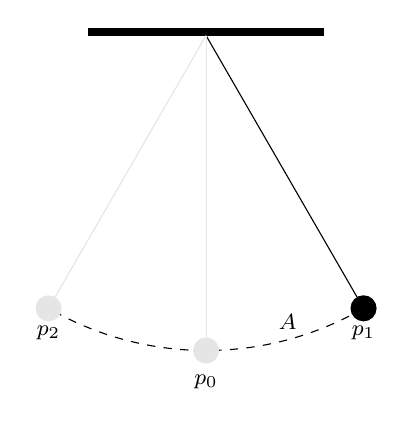
\begin{tikzpicture}[font=\footnotesize]

% Support
\fill (-1.5,0) rectangle(1.5,0.1);

% Bob's trajectory
	\draw[dashed]  (-60:4)  node[below,yshift=-.1cm]{$p_1$} arc (-60:-120:4) node[below,yshift=-.1cm]{$p_2$} node[midway,yshift=-.4cm]{$p_0$} ;
	
		\path  (-60:4) arc (-60:-90:4) node[midway,above]{$A$}; 

% Rod + Bob
\draw (0,0) -- (-60:4) node[fill,circle](m){} ;

% Weight Force
%\draw[-latex] (m) -- node[right]{$p_1$}++(0,-1) ;

% Tension Force
%\draw [-latex] (m) -- node[right]{$\vec{T}$}(-60:3);


% Light gray pendulum
\draw[black!10] (0,0) -- (-90:4) node[fill,circle]{};
\draw[black!10] (0,0) -- (-120:4) node[fill,circle]{};

\end{tikzpicture}

		\subcaption{Péndulo.}
		\label{fig:pendulo}
	\end{subfigure}
	\begin{subfigure}{0.4\textwidth}
		\begin{tikzpicture}[font=\footnotesize]
	\draw[-stealth] (4,0) -- (11.5,0) node[right ,font=\tiny] {$t$};
       \draw[stealth-] (5,2) node[above ,font=\tiny] {$A$} -- (5,-2);
  	%\draw[|-|, dashed] (6,0) -- (6,1)  node[midway,left ,font=\tiny] {$A$};
  	\draw[|-|, dashed] (5,-1) -- (9,-1)  node[midway,below ,font=\tiny] {$\lambda$};
  	%\draw (0.2,-1)node[left,font=\tiny] {$y=-1$} -- (11.8,-1); 
  	%foreach \x in {0,0.5,...,12}{
  	%	\draw (\x,-0.2)node [below,font=\tiny,] {\x} -- (\x,0.2) ;
  	%}
  	%\draw[] (3,0) sin (4,1);    %% the real business in this line
	\draw[lightgray,thick] (4,1) cos (5,0) node[black, below left] {{$p_0$}};    %% the real business in this line
  	\draw[thick] (5,0) sin (6,-1) node[black, below] {{$p_1$}};    %% the real business in this line
  	\draw[thick] (6,-1) cos (7,0)  node[black, below right] {{$p_0$}};    %% the real business in this line
  	\draw[thick] (7,0)  sin (8,1) node[black, above] {{$p_2$}};    %% the real business in this line
  	\draw[thick] (8,1) cos (9,0) node[black, below right] {{$p_0$}};    %% the real business in this line
  	\draw[lightgray,thick] (9,0) sin (10,-1);    %% the real business in this line
  	\draw[lightgray,thick] (10,-1) cos (11,0);    %% the real business in this line
\end{tikzpicture}

		\subcaption{Onda simple.}
		\label{fig:onda}
	\end{subfigure}
	\label{fig:ondapen}
	\caption{Descripción de la onda sonora.}
\end{figure}

La \textit{intensidad}\index{intensidad} ($I$) con la que percibimos el sonido en un punto es la cantidad de energía que atraviesa en sentido perpendicular la unidad de superficie colocada en ese punto por unidad de tiempo. En el sistema internacional esta magnitud se mide en $J/m^2 \cdot s$ o $w/m^2$; es proporcional al cuadrado de la amplitud y de la frecuencia. Es usual emplear también el \textit{decibelio}\index{decibelio}, una medida logarítmica definida por la intensidad de un sonido determinado ($I$) y una umbral ($I_0=10^{-12} w/m^2$), tal como se define en la ecuación \ref{beta}.
\begin{equation}\label{beta}
	\beta = 10 \cdot \log{\frac{I}{I_0}}
\end{equation}
Los fundamentos de la onda simple son la base conceptual para abordar el sonido lingüístico. Este es siempre una combinación de varias de estas ondas porque ni el aparato fonador humano es capaz de producir un sonido «puro» ni el medio de transmisión que encontraremos en circunstancias normales provee las condiciones para una propagación uniforme. Por lo tanto, el sonido lingüístico es una \textit{onda compleja}\index{onda!compleja|see {compuesta}} o \textit{compuesta}\index{onda!compuesta}, resultante de la adición de un número dado de ondas simples\index{onda!simple} (\Cref{fig:ondacompleja}). La distribución de las amplitudes de cada frecuencia simple de una onda compleja constituye el \textit{espectro} del sonido\index{espectro}.

\begin{figure}[!ht]
	\centering
		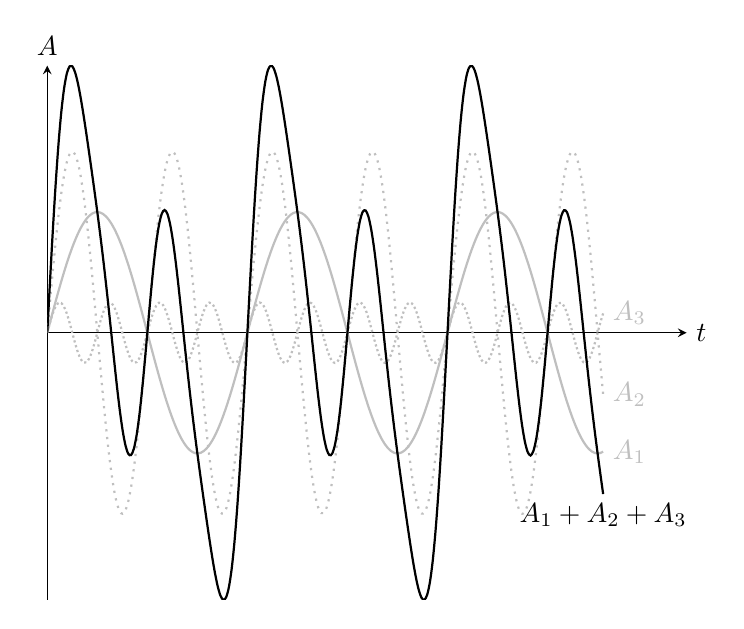
\begin{tikzpicture}[domain = 0:16, samples = 1000]
		%\draw[very thin, color = gray, step=1] (0,-2.75) grid(16,2.75);
		% zero crossing
		%\draw[dotted] (0,0) -- (16,0);
		%\draw (6.25,3) -- (6.25,-3) node[below] {$4ms$};
		\begin{axis}[
			width = 0.8\textwidth,
			axis x line=middle,
			axis y line=middle,
			ylabel = {$A$},
			ylabel style={at=(current axis.above origin), anchor=south}, 
			ytick=\empty,
			xtick=\empty,
				xlabel = {$t$},
				xlabel style={at=(current axis.right of origin), anchor=west},
				xmax=1150]	
		%	height = 0.5\textwidth]
		\addplot[thick, dotted, color=lightgray,
		domain = 0:1000,
		samples = 200,
		smooth]
	{sin(2*x)*1.5} node (b){};
	\node [right,color=lightgray] at (b) {$A_2$};
		\addplot[thick, color=lightgray,domain = 0:1000,
		samples = 200,
		smooth] plot[id=a]
	{sin(x)} node (a){};
	\node [right,color=lightgray] at (a) {$A_1$};
		\addplot[thick, color=lightgray, densely dotted,domain = 0:1000,
		samples = 200,
		smooth] plot[id=b]
	{sin(4*x)/4} node (c){};
	\node [right,color=lightgray] at (c) {$A_3$};
		\addplot[thick,id =d,domain = 0:1000,
		samples = 200,
		smooth]	{sin(4*x)/4 + sin(x) +  sin(2*x)*1.5}  node (y){};
		\node [below] at (y) {$A_1 + A_2 + A_3$};

\end{axis}
	\end{tikzpicture}

	\caption{Onda compleja y las ondas simples que la componen.}
	\label{fig:ondacompleja}
\end{figure}

Las ondas compuestas son \textit{periódicas}\index{onda!compuesta!periódica} o \textit{armónicas}\index{onda!compuesta!armónica|see {periódica}} y \textit{aperiódicas}\index{onda!compuesta!aperiódica} o \textit{inarmónicas}\index{onda!compuesta!inarmónica|see {aperiódica}}. En el primer caso, la frecuencia de cada una de las ondas simples es un múltiplo entero de la onda simple de frecuencia más baja, que denominamos \textit{frecuencia fundamental}\index{frecuencia!fundamental}. La onda correspondiente se conoce como \textit{primer armónico}\index{armónico} o tono fundamental. Al ser el resto de armónicos múltiplos del primero, la onda compleja se repite con la misma frecuencia que la onda simple de frecuencia más baja.  En \Cref{fig:ondacompleja} esta corresponde a la onda $a$. Las ondas $b$ y $c$ serían, respectivamente, el primer y el segundo armónico\index{armónico} de aquella. Este tipo de onda lo tienen todos los sonidos vocálicos. En el caso de las ondas aperiódicas, como las resultantes de producir \ipa{[f]} o \ipa{[s]}, la proporcionalidad no se cumple, por lo que el espectro del sonido no presenta la regularidad del tipo anterior. La impresión auditiva registrada de la frecuencia fundamental se denomina \textit{tono}\index{tono} y determina la \textit{entonación}\index{entonación} a nivel oracional. El número y la cualidad de los armónicos, por su parte, configuran el \textit{timbre}\index{timbre} \parencites[94]{quilis2019}[93]{clegg2018}. 

Llamamos \textit{resonancia acústica}\index{resonancia} al fenómeno en el que un cuerpo vibrante comunica esta vibración a otro cuerpo cercano. Se da cuando la frecuencia de la vibración del primer cuerpo coincide con la frecuencia natural de vibración del segundo  (\textit{resonador}\index{resonador}). La extensión del rango de frecuencias efectivas del resonador se denomina \textit{ancho de banda}\index{ancho de banda}. Aprovechando esta característica, es posible emplear el resonador como un \textit{filtro}\index{filtro} acústico, al amplificar solo determinadas frecuencias.

El sonido lingüístico se produce de tres maneras diferentes, tal como indica Quilis \parencite*{quilis2019}. Los sonidos sonoros son resultado del flujo de aire al atravesar la glotis\index{glotis} puesta en vibración. Otros sonidos se originan al paso de la corriente de aire por constricciones, tal y como sucede en las fricativas\index{consonante!fricativa}. Por último, la obstrucción del paso a través del conducto vocal produce una compresión  del aire que, al ser liberado, provoca una explosión, como en el caso de las consonantes oclusivas\index{consonante!oclusiva}.

El tracto vocal es un tubo cerrado en un extremo y de apertura regulable en el otro. Esto es, en uno de los dos finales de este canal, se encuentra la laringe, que bloquea la salida del aire; en el otro, se hallan dos salidas, la boca y las fosas nasales, cuya apertura o cierre cambia el hablante a discreción, pudiendo cerrarla completamente o graduar la apertura mediante el movimiento de la lengua o los labios. Las cavidades actúan asimismo como resonadores, cuyas frecuencias de respuesta se alteran desplazando los órganos articulatorios, de forma que estos, en función de su posición, filtren determinadas frecuencias y amplifiquen otras.

Los picos del espectro del sonido se denominan \textit{formantes}\index{formante}. Se ha observado experimentalmente que la resonancia encuentra un rango de frecuencias de transmisión efectiva en el tracto vocal, con independencia del origen del sonido. Esta frecuencia se encuentra muy próxima al máximo del espectro del sonido íntegro, por lo que, aunque sean diferentes desde un punto de vista conceptual, la frecuencia de resonancia y la del formante pueden ser consideradas equivalentes a efectos prácticos \parencite[20]{fant1970}.

\begin{figure}[!ht]
	\centering
	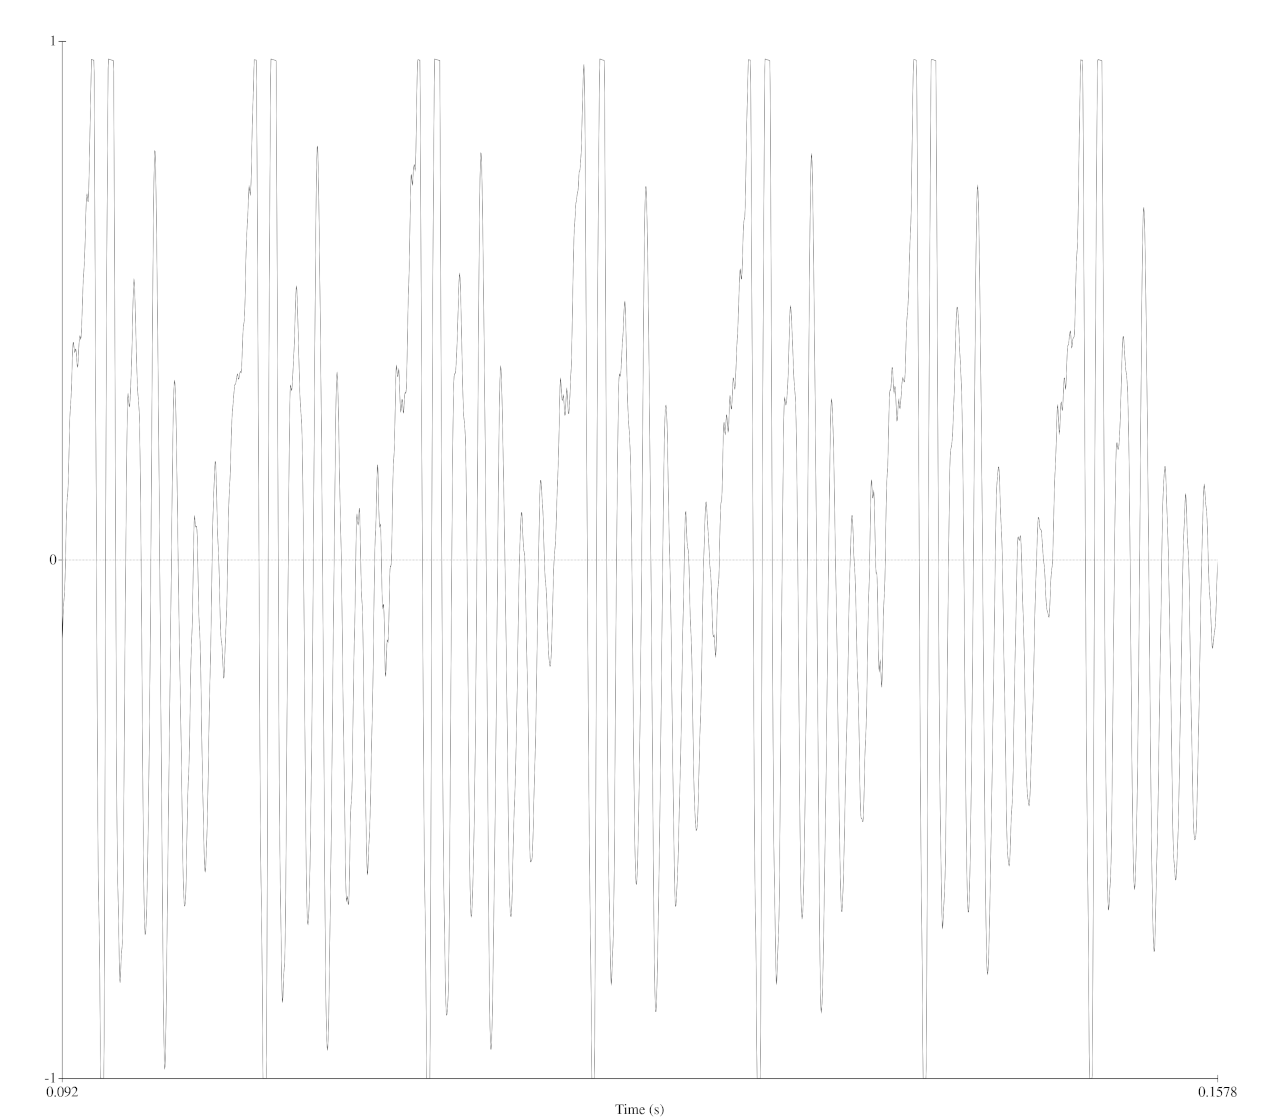
\includegraphics[width=0.75\textwidth]{images/ondaa}
	\caption{Onda de [aː].}
	\label{fig:ondaa}
\end{figure}

Con esto, emprendemos la tarea pertrechados de los medios técnicos apropiados \parencite{boersma2022}: analizar un \textit{sonograma}\index{sonograma} (\Cref{fig:sonogramas}), que es el gráfico que representa las variaciones de la frecuencia en el eje de ordenadas a lo largo del tiempo en el de abscisas. El sonograma se filtra según un determinado rango de frecuencias para examinar diferentes aspectos del sonido. Así, un sonograma \textit{de banda estrecha}\index{sonograma!de banda estrecha} como el de \Cref{fig:anarrow} es más adecuados para observar los armónicos de la onda, más difíciles de discernir en uno \textit{de banda ancha}\index{sonograma!de banda ancha} como el de \Cref{fig:awide}, que, por el contrario, ofrece una perspectiva más amplia del sonido \parencite[95-96]{clegg2018}. Las franjas más oscuras corresponden a los formantes\index{formante} en el sonograma de banda estrecha o a sus agrupaciones en el de banda ancha. En el ejemplo, que representa el sonido \ipa{/a/}, la frecuencia fundamental se encuentra alrededor de los 108,65 Hz, el primer formante $F_1$ tiene una frecuencia ocho veces mayor, el segundo $F_2$ diez veces mayor, el tercero $F_3$ veinticuatro veces mayor y el cuarto $F_4$  veinticinco veces más.

\begin{figure}[!ht]
	\centering
	\begin{subfigure}{0.49\textwidth}
		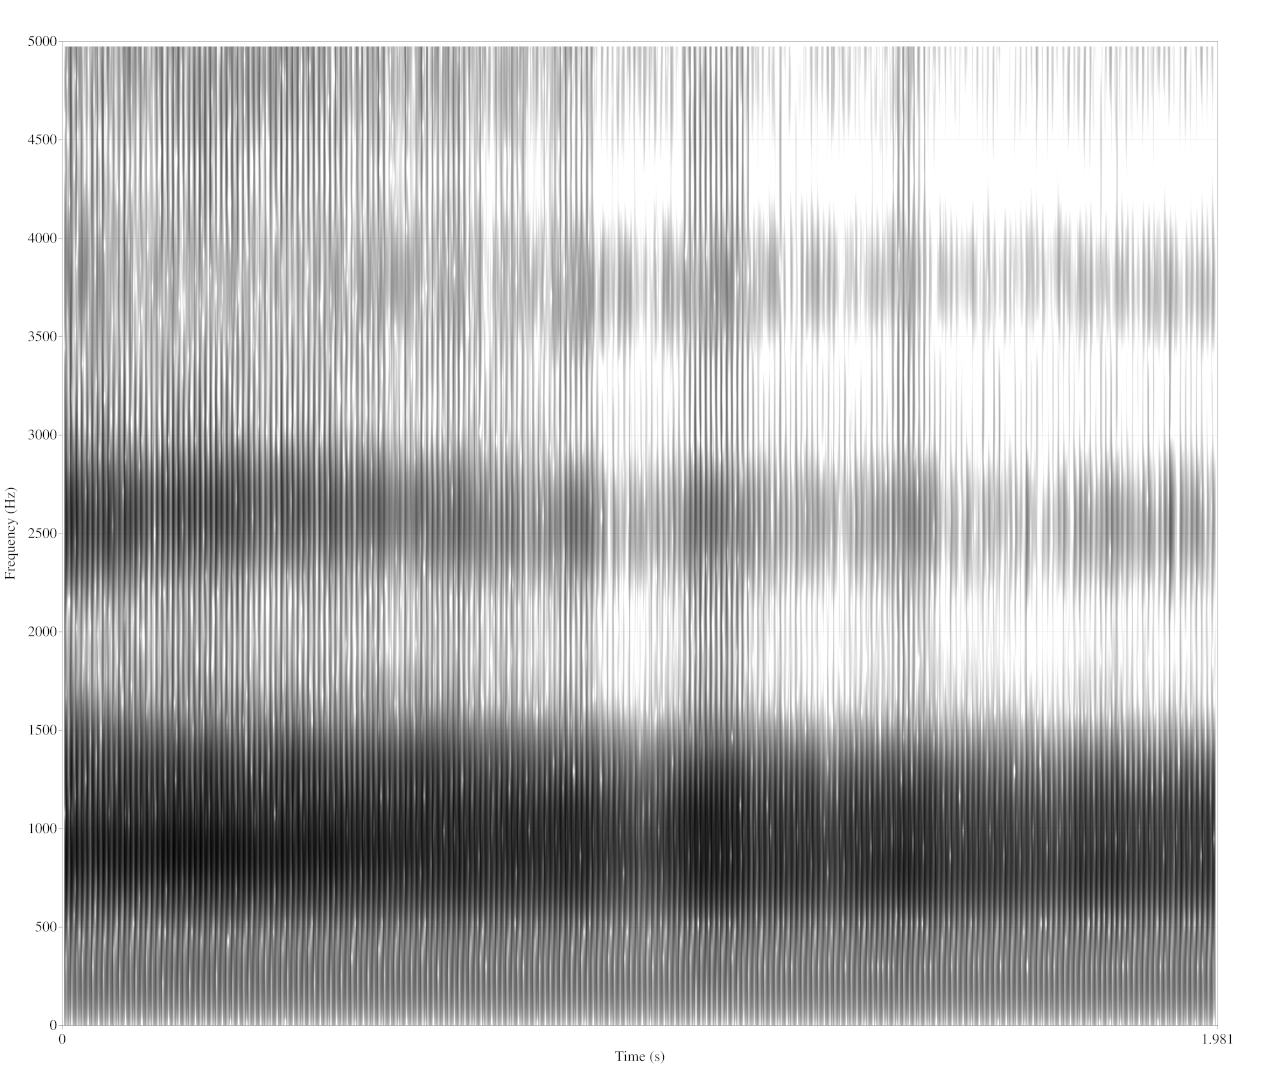
\includegraphics[width=\textwidth]{images/awidex}
		\subcaption{Banda ancha.}
		\label{fig:awide}
	\end{subfigure}
	\begin{subfigure}{0.49\textwidth}
		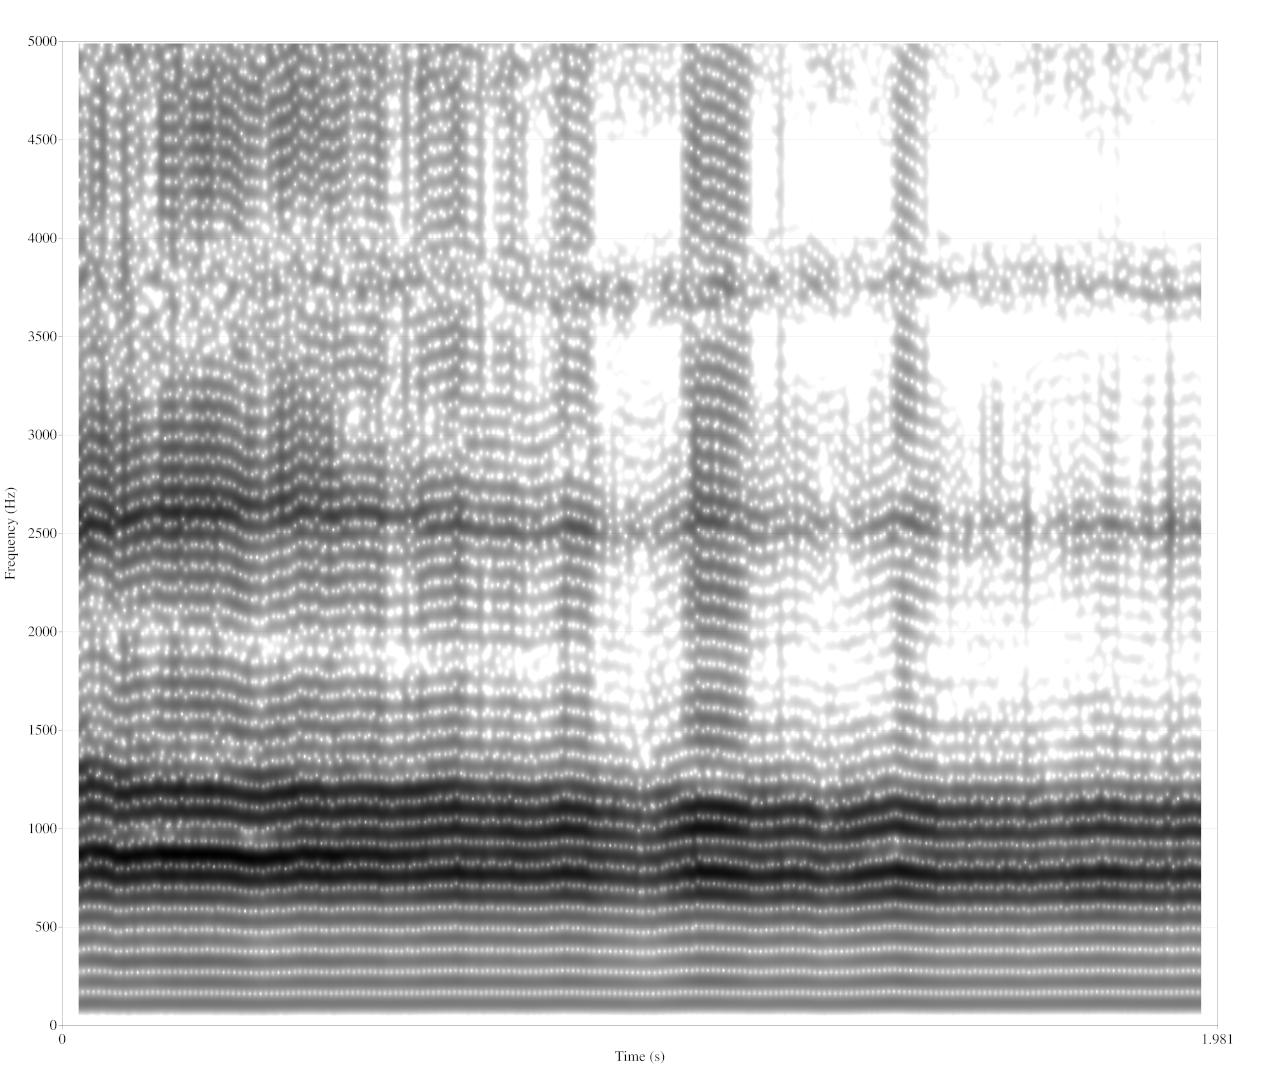
\includegraphics[width=\textwidth]{images/anarrowx}
		\subcaption{Banda estrecha.}
		\label{fig:anarrow}
	\end{subfigure}
	\caption{Espectrogramas de [aː].}
	\label{fig:sonogramas}
\end{figure}


Estos formantes\index{formante}, de forma especial el primero y el segundo, facilitan la distinción entre las vocales. El primer formante $F_1$ viene definido por la manera de articulación, ya que la frecuencia de este tiene una relación proporcional con la apertura bucal y, por el contrario,  cuanto más cerrada se encuentre la boca, tanto más bajo será el formante. El segundo formante lo determina el lugar de articulación, de manera que cuanto más anterior sea la articulación, más alta será la frecuencia y viceversa, cuanto más posterior sea el sonido, más baja la frecuencia de $F_2$. De esta manera, los valores de $F_1$ de las vocales españolas serían aproximadamente los representados en la Tabla \ref{tab:formantvocales} \parencite[101]{clegg2018}.

\begin{table}[!ht]
	\centering\small
	\begin{tikzpicture}[font=\footnotesize, domain=0:] %, every node/.style={fill, circle, inner sep = 1pt}]
    \begin{axis}[
    	 /pgf/number format/.cd,
    	use comma,
    	1000 sep={},
      width = 0.8\textwidth,
      axis lines = middle,
      xmin=700,
      xmax=2300,
      ymin=200,
      ymax=900,
      ylabel style={at=(current axis.below origin), anchor=south, , yshift=-0.5cm},
      x dir=reverse,
      y dir=reverse,  
      %label style={at=(current axis.below origin), anchor=south},
      xlabel style={at=(current axis.left of origin), anchor=west, xshift=-0.5cm},
      %xticklabel pos=right,
      %ylabel near ticks,
      % yticklabel pos=right,
      enlargelimits = true,
      xlabel={$F_2$},
      ylabel={$F_1$}],
    ]    
    \node (i) at (2174,315) {\large$i$};
    \node (e) at (1895,501) {\large$e$};
     \node (a) at (1300,762) {\large$a$};
    \node (o) at (966,501) {\large$o$};
     \node (u) at (836,315) {\large$u$};
    \end{axis}


  \end{tikzpicture}

	\caption{Formantes $F_1$ y $F_2$ de las vocales (Hz).}
	\label{tab:formantvocales}
\end{table}

La relación con el trapecio articulatorio se hace más evidente si disponemos estos valores en un gráfico. Como muestra \Cref{fig:formantvocales}, la posición de los sonidos según las frecuencias de sus dos primeros formantes\index{formante} está relacionada con el trapecio articulatorio.

Para interpretar sonidos consonánticos no basta con identificar el modo y lugar de articulación, sino que una descripción precisa requiere conocer el estado de las cuerdas vocales; esto es, hallar el grado de intervención de este órgano porque su vibración determina si la consonante es \textit{sonora}\index{consonante!sonora} o \textit{muda}\index{consonante!muda}.

Las oclusivas\index{consonante!oclusiva} se identifican por presentar un periodo de ausencia de energía durante la fase productiva, en el que no hay expulsión de aire. En las fricativas\index{consonante!fricativa}, la energía se extiende por el gráfico a lo largo del tiempo de producción. Las africadas\index{consonante!africada} están caracterizadas por la producción en dos fases, una primera oclusiva seguida de otra de liberación africada. Las consonantes nasales\index{consonante!nasal} y laterales\index{consonante!lateral}, conocidas también como \textit{sonorantes}\index{consonante!sonorante}, presentan formantes\index{formante} al modo de los sonidos vocálicos, aunque estos no son tan intensos. Las vibrantes\index{consonante!vibrante} se distinguen por las interrupciones de la onda sonora, poseyendo varias las múltiples\index{consonante!vibrante!múltiple} y una las simples \index{consonante!vibrante!simplel} \parencite[101-102]{clegg2018}.

\begin{figure}[!ht]
	\centering\small
	\begin{tikzpicture}[font=\footnotesize, domain=0:] %, every node/.style={fill, circle, inner sep = 1pt}]
    \begin{axis}[
    	 /pgf/number format/.cd,
    	use comma,
    	1000 sep={},
      width = 0.8\textwidth,
      axis lines = middle,
      xmin=700,
      xmax=2300,
      ymin=200,
      ymax=900,
      ylabel style={at=(current axis.below origin), anchor=south, , yshift=-0.5cm},
      x dir=reverse,
      y dir=reverse,  
      %label style={at=(current axis.below origin), anchor=south},
      xlabel style={at=(current axis.left of origin), anchor=west, xshift=-0.5cm},
      %xticklabel pos=right,
      %ylabel near ticks,
      % yticklabel pos=right,
      enlargelimits = true,
      xlabel={$F_2$},
      ylabel={$F_1$}],
    ]    
    \node (i) at (2174,315) {\large$i$};
    \node (e) at (1895,501) {\large$e$};
     \node (a) at (1300,762) {\large$a$};
    \node (o) at (966,501) {\large$o$};
     \node (u) at (836,315) {\large$u$};
    \end{axis}


  \end{tikzpicture}

	\caption{Formantes $F_1$ y $F_2$ de las vocales (Hz).}
	\label{fig:formantvocales}
\end{figure}	

La posición de la articulación varía con el  modo en que esta se produce\index{articulación!modo}. Para las oclusivas, hay que observar las transiciones entre formantes\index{formante} de las vocales en contacto con la consonante, ya que estas tienen formas propias para cada sonido. En el caso de las fricativas, hay que tener en cuenta además la energía acústica empleada en su producción \parencite[102]{clegg2018}. Determinar la sonoridad de la consonante presenta menos dificultades. La vibración de las cuerdas vocales se aprecia en el sonograma de banda ancha, que muestra estrías verticales en las sonoras\index{consonante!sonora}, de las que carecen las sordas\index{consonante!sorda} \parencite[102]{clegg2018}. 



%\begin{table}[!ht]
	%\centering\small
	%\input{tables/formantnasales}
	%\caption{Formantes de las consonantes nasales y laterales  (Hz).}
	%\label{tab:formantnasales}
%\end{table}



\section{El sistema fonológico}
La unidad fonológica mínima es el \textit{fonema}\index{fonema}, que Jakobson \parencite*[231]{jakobson1962a} define como «un conjunto de propiedades sonoras concurrentes usadas en una lengua dada para distinguir palabras de significado distinto». Esto es, los fonemas deben servir al hablante para discriminar entre una palabra y otra según el principio\index{principio de pertinencia} de pertinencia\index{pertinencia|see{principio de pertinencia}}; esto es, lo que distingue entre las propiedades esenciales y las contingentes en la diferenciación de significados. En palabras de Martinet \parencite*[45]{martinet1970}, \blockquote{le principe de pertinence nous permet de distinguer ce	qui, dans chaque langue ou chaque usage, est essentiel parce que distinctif, et ce qui est contingent, c'est-à-dire déterminé par le contexte ou diverses circonstances}.

Un fonema, sin embargo, no corresponde a un sonido único, ya que admite varias realizaciones fonéticas con diferentes sonidos. Estas dependen del estilo de habla o del contexto fonético concreto en el que aparecen. La diferencia entre sonidos responde a factores externos y no influye en la distinción de significados, por lo que esos sonidos no son sino variantes de un fonema dado \parencite[231]{jakobson1962a} o \textit{alófonos}\index{alófono}.  Así, los sonidos \ipa{[β]} y \ipa{[b]} son realizaciones diferentes del mismo fonema \ipa{/b/}, y se selecciona una u otra dependiendo del contexto fonético donde se produzca el fonema. Por lo tanto, aunque \textit{abocar} se pronuncie \ipa{[aβoˈkaɾ]} y \textit{embozar} \textipa{[emboˈθaɾ]}, la diferencia no se percibe como un sonido diferente, por lo que hablamos de un único fonema \ipa{/b/}.

Esto obliga a establecer criterios para distinguir entre un fonema y una realización alternativa de este. Trubetzkoy \parencite*[42-46]{trubetzkoy1939} propone para ello las siguientes cuatro reglas:
\begin{enumerate}[label=\Roman*]
	\item «Cuando dos sonidos de la misma lengua se dan exactamente en el mismo contexto fónico y pueden intercambiarse sin provocar una diferencia en el significado intelectual de la palabra, esos dos sonidos son solo dos variantes facultativas de un único fonema» \parencite[p. 42; traducción propia]{trubetzkoy1939}. 
	\item «Cuando dos sonidos se dan exactamente en la misma posición fónica y no pueden ser intercambiados sin alterar el significado de la palabra o hacerla irreconocible, estos dos sonidos son realizaciones de dos fonemas distintos» (p. 44; traducción propia).
	\item  «Cuando dos sonidos acústica o articulatoriamente emparentados de una lengua no se dan nunca en el mismo contexto fónico, se consideran como variantes combinatorias del mismo fonema» (pp. 44-45; traducción propia).
	\item «Dos sonidos, aunque cumplan las condiciones de la regla III, no deben ser considerados variantes del mismo fonema en la lengua en cuestión si estos pueden darse en posiciones adyacentes, esto es, como grupo fónico de una secuencia de sonidos en aquellas posiciones en las que, también, uno de los sonidos también puede aparecer aislado» (p. 46; traducción propia).
\end{enumerate}
Estas reglas se ven mejor mediante casos prácticos. Verbigracia, la regla I se aplica a los sonidos \ipa{[h]} y \ipa{[s]} del español meridional como alófonos de /s/. Vemos que \ipa{[ˈkasah]} y \ipa{[ˈkasas]} son formas intercambiables de realizar \textit{casas}. El ejemplo que dimos arriba de \ipa{/ˈgata/} y \ipa{/ˈkata/} es representativo de la regla II. La regla III alude a casos como el de los alófonos \ipa{[d]} y \ipa{[ð]} del fonema \ipa{/d/}, pues el primer sonido únicamente aparece detrás de pausa, consonante nasal o lateral, mientras que el segundo lo hace en el resto de casos, no haciéndolo en los que afectan al primero. Así, tenemos \ipa{[esˈpalda]} y \ipa{[esˈpaða]}. La regla IV es relevante en ejemplos como el de la  semiconsonante\index{vocoide} \ipa{[w]} y la semivocal \ipa{[u̯]} como variantes combinatorias de \ipa{/u/}, ya que, además de cumplir la regla III, no aparecen en posición contigua a \ipa{[u]}.
 
Los sonidos lingüísticos, empero, en muy contadas ocasiones aparecen aislados. Por el contrario, suelen ser el resultado de la combinación articulada de una secuencia. Esto no es impedimento para que se dé el caso opuesto. Lo que en apariencia son dos fonemas individuales contiguos pueden no serlo, sino constituir solamente uno. Por ello, se hace necesario distinguir entre fonemas simples adyacentes y fonemas complejos constituidos de una serie de sonidos. Trubetzkoy propone las siguientes seis reglas para hacerlo:
\begin{enumerate}[label=\Roman*]
	\item «Solo puede ser considerado como realización de un fonema individual la unión de sonidos cuyos componentes no se reparten entre dos sílabas en la lengua en cuestión» \parencite[p. 50; traducción propia]{trubetzkoy1939}.
	\item «Solo puede ser considerado como realización de un fonema individual una unión de sonidos producida por un movimiento articulatorio homogéneo o a través de la disolución progresiva de un complejo articulatorio»  (p. 51; traducción propia).
	\item «Solo puede ser considerado como realización de un fonema individual una unión de sonidos cuya duración no sobrepase la duración de la realización de otros fonemas de la lengua en cuestión» (p. 53; traducción propia).
	\item «Una unión de sonidos potencialmente monofonemática —esto es, que cumple las reglas I, II y III— debe ser considerada realización de un único fonema si se trata como un fonema individual\footnote{La tautología es del original: «\begin{textgerman}Eine potentiell monophonematische Lautverbindung (d.i. den Forderungen der Regel I—III entsprechende) Lautverbindung muß als Realisation eines einzigen Phonems gewertet werden, wenn sie als Einzelphonem behandelt wird [...]\end{textgerman}».}, esto es, si se da en aquellas posiciones en las que grupos fonemáticos no pueden ocurrir en la lengua en cuestión» (p. 53; traducción propia).
		\item «Una combinación de sonidos que cumpla las reglas de I a III debe ser considerada la realización de un fonema si esto produce simetría en el sistema fonológico»\footnote{He recurrido a otra edición \parencite{trubetzkoy1969} porque la regla V no aparece en el texto original \parencite{trubetzkoy1939}, pasando de la IV a la elaboración de la V, pero sin llegar a enunciarla.} \parencite[p. 59; traducción propia]{trubetzkoy1969}.
	\item «Si un componente de una unión fonemática potencial no pude ser evaluada como variante combinatoria de algún otro fonema de la lengua en cuestión, la unión de sonidos debe ser interpretada como un fonema individual» \parencite[p. 56; traducción propia]{trubetzkoy1939}. 
\end{enumerate}

Podemos aclarar estos puntos con algunos casos ilustrativos. Vemos que en el fonema \ipa{/ʧ/} del español hay una obstrucción que se libera para deshacerse luego en la fricativa. Sin embargo, sus componentes \ipa{[t]} y \ipa{[ʃ]} no se dividen entre dos sílabas como sí ocurre en otros idiomas como el alemán. Compárense las palabras de sendas lenguas \textit{hucha} y \textit{Lautschrift}, pronunciadas respectivamente como \ipa{/ˈu.ʧa/} y \textipa{/ˈlaʊt.ʃrIft/}. De esta manera, atendiendo a las reglas I y II, \ipa{[tʃ]} constituirían un único fonema complejo /\texttoptiebar{tʃ}/ en español pero dos fonemas simples \ipa{/t/} y \ipa{/ʃ/} en alemán. El equivalente a estos fonemas germanos lo tenemos en castellano con  \ipa{/ks/}, la pronunciación de \textit{x}. En \textit{facsímil}, por ejemplo, se distribuye en dos sílabas como \ipa{/fak.ˈsi.mil/}. Con respecto a la regla III, se ve en \textit{preeminente} que no se interpreta como \textipa{/pre:mi.ˈnen.te/}, pues contravendría la homogeneidad silábica del español —sin olvidar que la cantidad no es contrastiva en esta lengua—. Sobre la regla IV, Trubetzkoy propone el ejemplo de palabras alemanas como \textit{Zwei} o \textit{Pflanze}, que parecen contravenir la regla de que el alemán solo permite en ataque los segmentos de tres consonantes \ipa{[ʃtr]}, \ipa{[ʃpl]} y \ipa{[ʃpr]}; de esta manera, parece obligado evaluar los grupos \ipa{[ts]} y \ipa{[pf]} en ataque como fonémicos.

Partiendo de lo expuesto, recabamos el inventario de fonemas de una lengua dada. Para ello necesitamos, además, determinar el \textit{contenido fónico}\index{fonema!contenido fónico} de cada uno de ellos, esto es, sus propiedades distintivas. Dicho de otra manera, se requiere encontrar aquellas características comunes a todas las variantes de un mismo fonema \parencite[59]{trubetzkoy1939}. Por ejemplo, si describimos el fonema \ipa{/d/} como plosivo\index{consonante!plosiva}, sería adecuado para su realización \ipa{[d]}, pero excluiría otras realizaciones tan válidas como el aproximante\index{consonante!aproximante} \ipa{[ð]}. Por el contrario, resultaría inadecuado describirla solo como dental porque, aunque ambos alófonos lo cumplen, también lo hacen realizaciones de otros fonemas, como  \ipa{[t]} y \ipa{[θ]}. Es necesario, por lo tanto, indicar los rasgos relevantes: en el caso de \ipa{/d/}, dental sonoro.

El nivel fonológico constituye el material principal que conforma  los cimientos sobre los que se asienta la métrica. Sin embargo, no hay que dejar de lado del todo algunos aspectos de la lengua que hunden sus raíces en la fonética, de forma muy especial en el territorio de las vocales, donde la propiedad silábica del fonema representa un papel protagonista en la medida del verso. Debemos, pues, dilucidar el modo en el que el contexto fónico afecta a los fonemas individuales si esto altera la sustancia métrica del verso. Debemos hacer notar que esta disolución de las lindes entre los niveles fonético y fonológico no es extraña a la disciplina. Tanto Quilis \parencite*{quilis2019} como Alarcos Llorach, por ejemplo, clasifican hasta cierto punto los fonemas según criterios fonéticos.  Este último lo justifica arguyendo que \blockquote[{\cite[54]{alarcos1964}}]{hay que tener presente la diferencia entre fonología y fonética, a pesar de que en la práctica fonológica se utiliza la nomenclatura fonética por simplicidad. Esta está basada en las características articulatorias de los sonidos, aunque haya entre sus términos algunos puramente impresionísticos; por ser bien conocida, ofrece ventajas para la comprensión el aprovecharla en fonología.}

Una vez establecido el marco en el que definiremos el sistema fonológico y hechas las debidas prevenciones, queda por definir una serie mínima de rasgos identificativos\index{rasgo distintivo} u oposiciones\index{oposición}. Estos rasgos no solo deben distinguir a los términos de la oposición, sino que tienen que representar una cualidad común a ambos \parencite[68-87]{trubetzkoy1969}. Esto servirá para organizar el repertorio de todos los fonemas disponibles en una lengua en un sistema fonológico.

Atendiendo a la relación con el sistema fonológico, se distingue entre \textit{oposiciones bilaterales}\index{oposición!bilateral} y \textit{multilaterales}\index{oposición!multilateral}\footnote{También se conocen como \textit{unidimensionales} y \textit{pluridimensionales}, respectivamente.}, y \textit{oposiciones proporcionales}\index{oposición!proporcional} y \textit{aisladas}\index{oposición!aislada}. Llamamos \textit{oposiciones bilaterales} a aquellas en las que el \textit{tertium comparationis} es particular de los dos términos y no se da en otro término del mismo sistema fonológico. Las \textit{oposiciones multilaterales}, por su parte, son aquellas en las que la base de la comparación se da en otros términos. Quilis \parencite*[36]{quilis2019} ejemplifica la relación bilateral con los fonemas \ipa{/k/}-\ipa{/x/} del español, cuyas propiedades compartidas (orales, velares, sordas) no aparecen juntas en ningún otro fonema, de la misma manera que \ipa{/e/}-\ipa{/i/} (vocales, sonoras, anteriores). Como ejemplo de multilateralidad, Quilis cita /b/-/d/, ya que sus rasgos comunes\index{rasgo distintivo} (consonantes, oclusivas, orales, sonoras) se dan también en /b/-/g/ o /d/-/g/.

En las \textit{oposiciones proporcionales}\index{oposición!proporcional}, la relación que se da entre sus términos se encuentra en los de otra oposición, mientras que los términos de las \textit{oposiciones aisladas} tienen una relación única en el sistema fonológico. De esta manera, /p/-/b/ es proporcional porque la misma relación se da en /t/-/d/ y /k/-/g/, mientras que la oposición /r/-/l/ es aislada, ya que la relación no aparece en ningún otro par del sistema. 

Según las relaciones entre los términos, las oposiciones son \textit{privativas}, \textit{graduales} o \textit{equipolentes}. Las \textit{oposiciones privativas}\index{oposición!privativa} son de naturaleza binaria y se caracterizan por la presencia o ausencia de una marca. El término que presenta la marca se denomina \textit{término marcado}\index{término!marcado} y, de forma análoga, el que no la presenta se llama \textit{no marcado}\index{término!no marcado}. Por ejemplo, si consideramos el rasgo sonoridad\index{rasgo distintivo}, en la oposición /p/-/b/, /b/ será el término marcado (sonoridad: +) y /p/ el no marcado (sonoridad: $-$). Por el contrario, las \textit{oposiciones graduales}\index{oposición!gradual} presentan la distinción como un grado no binario. La apertura de las vocales es un ejemplo de este tipo de oposiciones. Así, /i/ es más cerrada que /e/, que a su vez es más cerrada que /a/. Las \textit{oposiciones equipolentes}\index{oposición!equipolente} son aquellas cuyos miembros son equivalentes. Esto es, no han de ser consideradas ni privativas ni graduales, por ejemplo /p/-/k/ o /i/-u/.

Las oposiciones fonológicas también se caracterizan mediante su poder distintivo en \textit{constantes}\index{oposición!constante} o \textit{neutralizables}\index{oposición!neutralizable}. Las primeras se realizan siempre sin que tenga relevancia la posición que ocupen, mientras que las segundas no se dan en ciertas posiciones. En este último caso, la posición donde se mantiene la distinción se denomina \textit{de pertinencia}\index{posición!de pertinencia}, mientras que aquella en la que se neutraliza se llama \textit{de neutralización}\index{posición!de neutralización}. Por ejemplo, /s/-/θ/ serían constantes en \textit{español de Castilla}\footnote{Por comodidad, me referiré al español de Castilla para denotar las variedades peninsulares septentrionales que se acercan a lo que, con todas las precauciones, podríamos llamar \textit{español estándar}.} porque no pierden capacidad distintiva según su posición, como se ve en \textit{casa} /ˈka.sa/ y \textit{caza} /ˈka.θa/ o \textit{hez} /eθ/ y \textit{es} /es/. Por el contrario, /r/-/ɾ/ solo funcionan en posición prenuclear, de forma que mientras que \textit{perro} /ˈpe.ro/ y \textit{pero} /ˈpe.ɾo/ son distintas fonológicamente,  /baɾ/ y /bar/ son dos formas de pronunciar la misma palabra \textit{bar}.

Los rasgos distintivos\index{rasgo distintivo} varían según desde qué perspectiva fonética se aborde la fonología. Quilis \parencite*[44]{quilis2019} menciona la \textit{fonética sincrónica}\index{fonética!sincrónica}, \textit{diacrónica}\index{fonética!diacrónica}, \textit{articulatoria}\index{fonética!articulatoria}, \textit{acústica}\index{fonética!acústica}, \textit{auditiva}\index{fonética!auditiva} y \textit{psicológica}\index{fonética!psicológica}. Este estudio se vale ante todo de la fonética articulatoria\index{fonética!articulatoria} como marco descriptivo del sistema fonológico. Sin embargo, dadas las dificultades que presentaría examinar físicamente a los hablantes para controlar la producción del sonido, nos apoyaremos en la fonética acústica\index{fonética!acústica} para contrastar muestras de sonidos mediante la observación de sus espectrogramas. Esto permite, por un lado, obtener de manera sencilla las muestras como archivos de audio y, por otra parte, examinarlos a fondo con el \textit{software} adecuado\footnote{En nuestro caso, Praat \parencite{boersma2022}.}. Así pues, habremos de establecer estos marcos fonéticos descriptivos. 

Los rasgos distintivos\index{rasgo distintivo} en se dividen en \textit{prosódicos}\index{rasgo distintivo!prosódico} e \textit{intrínsecos}\index{rasgo distintivo!intrínseco} o \textit{inherentes}\index{rasgo distintivo!inherente|see {intrínseco}}. Todos los fonemas poseen estos últimos, pero los primeros son exclusivos de los fonemas constituyentes de núcleo silábico \parencite[111]{quilis2019}.

Desde un punto de vista acústico, se distinguen diferentes rasgos\index{rasgo distintivo}. Alarcos~Lorach~\parencite*[85]{alarcos1964} propone \textit{vocálico}/\textit{no vocálico} y \textit{consonántico}/\textit{no consonántico}, que se basan en el formante\index{formante} generador de la onda sonora y la presencia o ausencia de obstáculo en el canal bucal. Permiten discriminar entre fonemas vocales, consonantes, líquidos y glotales;  \textit{denso}/\textit{difuso}, basándose en la proporción de las cavidades bucofaríngeas; \textit{grave}/\textit{agudo}, junto a los rasgos precedentes\index{rasgo distintivo},  revela la ubicación de los fonemas, \textit{bemolizado}/\textit{normal} y  \textit{sostenido}/\textit{normal}, que dependen del timbre del resonador bucal y distinguen series paralelas de sonidos con timbre modificado; \textit{nasal}/\textit{oral}, según se emplee la nariz o la boca como cavidad resonadora; \textit{tenso}/\textit{flojo}, en función de la tensión de los órganos fonadores, que indica propiedades prosódicas de las vocales y distingue entre consonantes fuertes y débiles;  \textit{sonoro}/\textit{sordo}, que viene determinado por la vibración de la glotis y actúa en combinación con el rasgo precedente\index{rasgo distintivo}; \textit{continuo}/\textit{interrupto} y  \textit{estridente}/\textit{mate}, que dependen de si el ataque es abrupto o hay una interrupción en el flujo del aire, así como de la aproximación de los órganos fonadores y \textit{recursivo}/\textit{infraglotal}, determinado por la existencia de cierre glotal al final del sonido y diferencia el modo en que la glotis interviene en la expulsión del aire. 

Quilis \parencite*[165-167]{quilis2019}, por su parte, distingue para los sonidos vocálicos entre \textit{compactos} y \textit{no compactos}, siendo \textit{difuso} y \textit{no difuso} propiedades de los últimos. Asimismo, desdobla grave/agudo en \textit{grave} y \textit{no grave}, pudiendo aquellos que se hallan en el segundo caso subdividirse en \textit{agudo} y \textit{no agudo}. Además, hace distinciones más finas, añadiendo \textit{denso}/\textit{no denso}, \textit{difuso}/\textit{no difuso}, \textit{grave/no grave} y \textit{agudo/no agudo}.

\section{Neutralización}
El fenómeno de la neutralización\index{neutralización} consiste en la desaparición del contraste fonémico en ciertos entornos fonológicos, bien por la pérdida de una característica propia del fonema o por la adquisición de otra ajena a este. 

\citeauthor{alarcos1964}~\parencite*[97-99]{alarcos1964} describe dos tipos de neutralización, una \textit{condicionada por el contexto}\index{neutralización!condicionada} y otra \textit{exigida por la estructura}, que es \textit{interna}\index{neutralización!interna} del sistema. Mientras que la primera ocurre como respuesta a fonemas cercanos, como en el caso de una consonante nasal ante otra consonante, la segunda la determina la posición, como en las vibrantes a final de sílaba. La neutralización condicionada es \textit{disimilativa}\index{neutralización!disimilativa} si el fonema pierde su carácter distintivo por la influencia de otro con un rasgo distintivo semejante o \textit{asimilativa}\index{neutralización!asimilativa} si lo pierde por contacto con otros fonemas carentes de este. La neutralización interna, por su parte, se divide entre la \textit{centrífuga}\index{neutralización!centrífuga} y la \textit{reductiva}\index{neutralización!reductiva}. La neutralización centrífuga es aquella que ocurre en los límites de palabra o sílaba, mientras que la reductiva es la que se da en todas las sílabas menos en la culminante o acentuada.

Este suele darse con mayor frecuencia en la distensión silábica de final de sílaba \parencite[180]{alarcos1964}, lo que, a efectos prácticos, reduce su alcance a las consonantes que suelen darse en tal posición. En español, la neutralización es especialmente notable en coda. En lo que a nuestro estudio respecta, la asimilación en coda en la rima podría determinar la diferencia entre consonancia y asonancia. Esto, sin embargo, solo sucedería en casos tan excepcionales que podemos pasarlo por alto. No obstante, hemos de mencionarlo como una posibilidad teórica.

\section{Fonemas del español}
\subsection{Sonidos vocálicos}
Desde las gramáticas más primitivas de Grecia y la India, los estudiosos del lenguaje han divido los sonidos entre consonantes y vocales. Esta clasificación no es arbitraria, ya que se ha comprobado que hay diferencias articulatorias que, a su vez, tienen consecuencias en el plano acústico. Las vocales se producen por una acción articulatoria fuerte, en la que se alcanza una máxima apertura, mientras que una acción articulatoria débil produce el efecto contrario \parencite[141-143]{quilis2019}. En lo que concierne a este trabajo, los sonidos vocálicos son fundamentales, ya que con ellos se contarán las sílabas. Por esta razón debemos identificarlos y caracterizarlos. Sin embargo, aunque todos los núcleos silábicos son vocálicos, no todas las vocales  son necesariamente silábicas, por lo que será preciso, en ese caso, no solo caracterizarlas, sino identificar sus propiedades físicas para contar con criterios para resolver casos dudosos.

Podemos caracterizar los sonidos vocálicos, al igual que los consonánticos, por el modo\index{articulación!modo} y por el punto de articulación\index{articulación!punto}. El modo de articulación se refiere a la apertura que deja la lengua en la cavidad bucal, mientras que el punto de articulación, al contrario que las consonantes, no es respecto a cierres o puntos de contacto, sino a la región palatal a la que se aproxima el dorso lingual. Por el modo de articulación, distinguimos entre vocales altas, medias y bajas.

La lengua castellana se caracteriza por la homogeneidad del repertorio vocálico en todas sus variedades dialectales. Así se ha descrito tradicionalmente y la fonética moderna tampoco ha encontrado más vocales a nivel fonológico, por lo que limita a describir las diferentes realizaciones fonéticas de los fonemas. En la conciencia lingüística del hablante existen tan solo cinco vocales: \textit{a}, \textit{e}, \textit{i}, \textit{o} y \textit{u}. En este caso, sí existen alófonos que dependen sobre todo del contexto fónico del segmento dado \parencite[32]{navarrotomas1946}. Las realizaciones de \textipa{/a/}, \textipa{/e/} y \textipa{/o/} son siempre vocálicas puras y son capaces de formar núcleo vocálico, mientras que, como detallamos abajo, \textipa{/i/} y \textipa{/u/} se realizan como vocales puras cuando son tónicas o cuando son átonas, pero no están en contacto con otra vocal \parencite[152-153]{alarcos1964}.

Si nos situamos en el trapecio bucal, el fonema /i/ es articulatoriamente \textit{alto} y el más \textit{anterior} del repertorio español. Es acústicamente \textit{vocálico}, \textit{no consonántico}, \textit{no compacto}, \textit{difuso}, \textit{no grave} y \textit{agudo}. Presenta dos realizaciones en distribución complementaria. La primera es la oral regular [i] (\textlangle{}piso\textrangle{} [ˈpiso]). La segunda es la nasalizada [ĩ], cuando /i/ se encuentra entre pausa y consonante nasal (\textlangle{}instante\textrangle{} [ĩnsˈtan̪te]) o entre dos consonantes nasales (\textlangle{}mimo\textrangle{} [ˈmĩmo]) \parencite[168-169]{quilis2019}.

También localizada articulatoriamente en una posición anterior, aunque a una altura \textit{media}, se encuentra el fonema /e/. Acústicamente, se describe como vocálico, no consonántico, no compacto, \textit{no difuso}, no grave y agudo. Tiene también dos realizaciones, una oral regular \ipa{[e]} (\textlangle{}peso\textrangle{} \ipa{[ˈpeso]}), y otra  nasal \ipa{[ẽ]} cuando /e/ se encuentra entre pausa y consonante nasal (\textlangle{}encono\textrangle{} \ipa{[ẽŋˈkono]}) o entre dos consonantes nasales (\textlangle{}memo\textrangle{} \ipa{[ˈmẽmo]}) \parencite[169]{quilis2019}.

El fonema vocálico más \textit{central} y \textit{bajo} es \ipa{/a/}. Acústicamente, es vocálico, no consonántico, \textit{compacto}, \textit{denso}, no grave y \textit{no agudo}. También \ipa{/a/} presenta dos alófonos en distribuciones complementarias, uno nasal [ã] cuando se halla entre una pausa y una consonante nasal (\textlangle{}antena\textrangle{} \ipa{[ãn̪ˈtena]}) y otra regular \ipa{[a]} (\textlangle{}casa\textrangle{} \ipa{[ˈkasa]}) en el resto  \parencite[169]{quilis2019}.

El fonema /o/ es medio y \textit{posterior}. Conforme a sus propiedades acústicas, es vocálico, no consonántico, no compacto, no difuso, \textit{grave}. De la misma manera, \ipa{/o/} tiene dos realizaciones, una oral regular \ipa{[o]} (\textlangle{}vaso\textrangle{} \ipa{[ˈBaso]}) y otra  nasal \ipa{[õ]}, cuando /o/ se encuentra entre pausa y consonante nasal (\textlangle{}oncología\textrangle{}  \ipa{[õŋkoloˈxia]}) o entre dos consonantes nasales (\textlangle{}nona\textrangle{} \ipa{['nõna]}) \parencite[169]{quilis2019}.

Por último, el fonema \ipa{/u/} es articulatoriamente alto y posterior. Se caracteriza acústicamente por ser vocálico, no consonántico, no compacto, difuso, grave. Al igual que el resto de vocales, \ipa{/u/} también tiene dos realizaciones en distribución complementaria, una oral regular \ipa{[u]} (\textlangle{}huso\textrangle{} \ipa{['uso]}) y otra  nasal \ipa{[ũ]}, cuando \ipa{/u/} se encuentra entre pausa y consonante nasal (\textlangle{}ungüento\textrangle{} \ipa{[ũŋˈgwen̪to]}) o entre dos consonantes nasales (\textlangle{}mundo\textrangle{} \ipa{[ˈmũn̪do]}) \parencite[170]{quilis2019}.

Esto se resume en  que, considerando la apertura\index{articulación!modo}, el español tiene dos vocales \textit{altas}\index{vocal!alta} o \textit{cerradas}\index{vocal!cerrada}, aquellas en que la lengua se aproxima al paladar duro o al paladar blando. Estos son los fonemas \ipa{/i/} y \ipa{/u/}. También cuenta con dos vocales \textit{medias}\index{vocal!media}, en las que la lengua se separa de la bóveda del paladar para posicionarse en medio de la cavidad bucal. Estas son \ipa{/e/} y \ipa{/o/}. El español solo posee una vocal \textit{baja}\index{vocal!baja} o \textit{abierta}\index{vocal!abierta}, esto es, cuando se produce una apertura máxima al alejarse la lengua del paladar en el mayor grado colocándose en la parte inferior de la cavidad bucal. Esta es /a/ \parencite[146-147]{quilis2019}.

Según el punto  de articulación\index{articulación!punto}, el español dispone de vocales anteriores, centrales y posteriores. Las vocales anteriores\index{vocal!anterior}, aquellas que se producen cuando la lengua se halla en la parte frontal de la cavidad bucal, son /i/ y /e/. En español solo aparece \textipa{/a/} como vocal media, en la que el dorso de la lengua se halla en la región del paladar medio\index{vocal!central}. Las vocales posteriores del español, en las que el posdorso de la lengua se acerca a la región posterior de la cavidad bucal, son /u/ y /o/ \parencite[147-148]{quilis2019}. En lo relativo a sus cualidades acústicas, todas las vocales del repertorio fonológico del español son \textit{vocálicas} y \textit{no consonánticas}.

\begin{table}[h!]
	\centering\small
	\begin{tabular}{lccc}
		\toprule	
		& \textbf{Anterior} & \textbf{Central} & \textbf{Posterior}  \\
		\midrule
		\textbf{Cerrada}          &  i  &   & u    \\
		\textbf{Media}       & e̞  &   &o̞   \\
		\textbf{Abierta}       &     & ä  &   \\
		\bottomrule
	\end{tabular}
	\caption{Fonemas vocálicos del español.}
	\label{tab:vocales}
\end{table}


Así pues, la lengua española cuenta con cinco vocales\index{vocal} que se distinguen entre sí por oposición: la anterior cerrada /i/, la anterior media /e/, la central abierta /a/, la posterior cerrada /u/ y la posterior media /o/. Todas ellas aparecen indistintamente en posición tónica\index{sílaba!tónica} (\ref{ex:dado}) y átona\index{sílaba!átona} (\ref{ex:dato}).

\begin{table}[!ht]
	\centering\small
	\begin{tabular}{lccccc}
		\toprule
		Rasgos&i&e&a&o&u\\
		\midrule
		Vocálico/no vocálico&+&+&+&+&+\\
		Consonántico/no consonántico&-&-&-&-&-\\
		Compacto/no compacto&-&-&+&-&-\\
		Difuso/no difuso&+&-&-&-&+\\
		Grave/no grave&-&-&-&+&+\\
		Agudo/no agudo&+&+&-&-&-\\
		\bottomrule
	\end{tabular}
	\caption{Rasgos acústicos de las vocales del español.}
	\label{tab:vocales-acusticas}
\end{table}



Aunque desde una perspectiva fonológica, determinados alófonos\index{alófono} de la lengua estándar representan fonemas por sí mismos en algunos dialectos, no nos ocuparemos de esas variedades diatópicas; nos centraremos en la estándar. Esto es, no consideraremos que, por ejemplo, en algunas variedades meridionales, la cualidad vocálica tiene valor fonológico y la apertura de /e/ es contrastiva. En esas variedades, \ipa{[ˈpaðɾɛ]} no es equivalente a \ipa{[ˈpaðɾe]} porque, mientras que esta última realización se estaría refiriendo al singular \textlangle{}padre\textrangle{}, la primera lo haría al plural \textlangle{}padres\textrangle{}. Por el contrario, en el español estándar \ipa{[ɛ]} y \ipa{[e]} son alófonos del fonema \ipa{/e/}, por lo que ambas realizaciones corresponderían a \textlangle{}padre\textrangle{} \parencites[148-150]{alarcos1964}[173-176]{quilis2019}. Por esto, sintetizamos el sistema vocálico ideal en los cinco fonemas \ipa{/a/}, \ipa{/e/}, \ipa{/i/}, \ipa{/o/} y \ipa{/u/}, sin contemplar variaciones no distintivas en la cualidad.

\begin{exe}  
\ex\label{ex:dado} /ˈdado/\tab\textit{dado} \\
 /ˈdedo/\tab\textit{dedo}\\ 
 /ˈdido/\tab\textit{Dido}\\
  /ˈdodo/\tab\textit{dodo}\\
  /ˈdudo/\tab\textit{dudo} 
\ex\label{ex:dato}  /daˈto/\tab\textit{dató} \\
/deˈxo/\tab\textit{dejó}\\ 
/diɾiˈxjo/\tab\textit{dirigió} \\
 /doˈljo/\tab\textit{dolió} \\
  /duˈdo/\tab\textit{dudó}
\end{exe}

A consecuencia de lo expuesto, los fonemas \ipa{/a/}, \ipa{/e/}, \ipa{/i/}, \ipa{/o/} y \ipa{/u/} se relacionan biunívocamente con los grafemas\index{grafema}  \textlangle{}a\textrangle{}, \textlangle{}e\textrangle{}, \textlangle{}i\textrangle{}, \textlangle{}o\textrangle{} y \textlangle{}u\textrangle{}, salvando las excepciones de los dígrafos\index{dígrafo} \textit{gu-} y \textit{qu-}. En esos casos, se trata de una sola unidad cuyos componentes no tienen realización fonológica propia independiente. Sin embargo, esto no es suficiente en el análisis métrico porque la cuenta de vocales silábicas\index{vocal!silábica} es lo que determina en último término el cómputo silábico del verso.

Dicho de otra manera, únicamente los fonos silábicos son relevantes en el cómputo de sílabas del verso con independencia de su función fonológica. Por ejemplo, la palabra \textlangle{}hueco\textrangle{} se analizaría fonológicamente como \ipa{/ˈue.ko/}. Si no atendemos al valor silábico de las vocales, tendríamos tres sílabas alrededor de los núcleos \ipa{/u/}, \ipa{/e/} y \ipa{/o/}. Sin embargo, este no es el caso, pues solo son silábicas \ipa{/e/} y \ipa{/o/}. Aquí, el fonema /u/ se une a \ipa{/e/} como semiconsonante no silábica, formando un diptongo en \ipa{[ˈwe.ko]}. De la misma manera, \textlangle{}hoy\textrangle{} se transcribiría \ipa{/oi/}, a pesar del diptongo en el que /i/ se realiza como una semivocal \ipa{[oi̯]}. Si vamos a ocuparnos de las sílabas, bien podemos añadir vocoides\index{vocoide} no silábicos a nuestro repertorio,  las semivocales \ipa{[u̯]} e \ipa{[i̯]}\index{semivocal} y las semiconsonantes \ipa{[w]} y \ipa{[j]}\index{semiconsonante} como realizaciones en posición no vocálica de \textlangle{}u\textrangle{} e \textlangle{}i\textrangle{}, respectivamente. Como veremos más adelante, en métrica, esta propiedad no se circunscribe a los diptongos naturales del español, sino que, estando dos vocales cualesquiera en contacto, una de ellas pierde su condición silábica en determinadas circunstancias y altera el número de sílabas del verso\index{sinalefa}.

Respecto a las diferencias fonéticas en la realización de los alófonos vocálicos, estas no influyen en la constitución métrica esencial del verso ni en apoyos secundarios, como la armonía vocálica. No obstante, la ausencia de relevancia métrica no implica que no aporten matices al verso. Cabe suponer que diferentes sonidos confieren un tono particular a las palabras. De ser así, habría que considerar en qué medida estaría esto provocado por la vocal o por el entorno fónico concreto que determina un alófono dado.
 
\subsection{Secuencias vocálicas}\label{sec:diptongo}
Una secuencia\index{secuencia vocálica} de dos o más vocales se da en una sola sílaba, lo que llamamos diptongo\index{diptongo} o un triptongo\index{triptongo}, o distribuida en sílabas diferenciadas, lo que constituye un hiato\index{hiato}. En el primer caso, tenemos palabras como \textlangle{}ay\textrangle{} /ai/ y \textlangle{}buey\textrangle{} /buei/, y en el segundo \textlangle{}ahí\textrangle{} /aˈi/. 

Los diptongos\index{diptongo} en español suelen aparecer como la recategorización de un hiato\index{hiato} \parencite{chitoran2007}. El fenómeno surge de forma natural en el habla rápida y descuidada cuando se encuentran dos vocales. En este caso, se funden en un único sonido si se trata de dos instancias del mismo fonema, mientras que, uno de ellos deviene en no silábico si son dos vocales distintas. De esta manera, \textlangle{}creer\textrangle{} se realiza como \ipa{[kɾeɾ]} y  \textlangle{}avión\textrangle{} como \ipa{[aˈBjon]}\footnote{Además de este fenómeno natural, debemos mencionar otro artificial de la misma índole consistente en la prescripción institucional de diptongos arbitrarios contra el uso habitual. Así, palabras como \textlangle{}cruel\textrangle{}, cuya forma bisilábica es la común y aceptada en el solar natal de la lengua castellana \parencite[185-186]{quilis2019}, obligarían a considerar excepciones en el sistema de representación propuesto por la Academia de querer amoldar el modelo al referente real. En lugar de eso, se optó por tratar de adaptar la lengua a su modelo.}.

Se ha discutido si los diptongos tienen un carácter monofonemático, como defiende \citeauthor{navarrotomas1946}~\parencite*[13-14]{navarrotomas1946}. Se apoya en las reglas I, II y III de Trubetzkoy \parencite*[42-45]{trubetzkoy1939} para determinar la naturaleza fonemática de un sonido, pero la postura contraria \parencite[§ 96]{alarcos1964} parece tener más peso, ya que se incumplen los puntos I y II, que son propios de un sonido monofonemático. Si tenemos en cuenta los requisitos que también propone Trubetzkoy \parencite*[50-52]{trubetzkoy1939} para verificar la naturaleza monofonemática de un sonido, hemos de descartar la tesis de Navarro Tomás.

A nivel fonológico,  solo hablamos de diptongos propios cuando es una vocal cerrada la que pierde el carácter silábico. De esta forma, el español cuenta con un repertorio de seis diptongos crecientes\index{diptongo!creciente} (vocal\textsuperscript{$+\textsc{cerrada}$} vocal\textsuperscript{$-\textsc{cerrada}$}),  siete decrecientes\index{diptongo!decreciente} (vocal\textsuperscript{$+\textsc{cerrada}$} vocal\textsuperscript{$-\textsc{cerrada}$}) y dos homogéneos\index{diptongo!homogéneo} (vocal\textsuperscript{$+\textsc{cerrada}$} vocal\textsuperscript{$-\textsc{cerrada}$}). En el último caso, la primera vocal pierde la naturaleza silábica y es la segunda la que hace de núcleo \parencite{quilis2019}. Cabe mencionar la particularidad de que, en caso de que la semiconsonante \textipa{[w]} sea el primer alófono prenuclear de la sílaba, es corriente la anteposición de un alófono de \textipa{/g/} (p. ej., \textlangle{}hueso\textrangle{} \textipa{/ˈgwe.so/}).

\begin{table}[h!]
	\centering\small
	\begin{tabular}{rcccccc}
		\toprule
		& \textbf{Tipo} & \textbf{V$_1$} & \textbf{V$_2$} & \textbf{Ejemplo} & \textbf{t. fonológica} & \textbf{t. fonética} \\
		\midrule
		1& $\nearrow$ &/i/  &	/e/  &    \textit{tiene} &	/ˈtie.ne/  &	[ˈt̪je.ne]  \\
		2& $\nearrow$ &/i/  &	/a/  &   \textit{patria} &	/ˈpa.tɾia/  &	[ˈpa.t̪ɾja] \\
		3& $\nearrow$ &/i/  &	/o/   &       \textit{vio} &	/ˈbio/  &	[ˈbjo]  \\
		4& $\nearrow$ &/u/  &	/e/  &  \textit{bueno} &	/ˈbue.no/  &	[ˈbwe.no] \\
		5& $\nearrow$ &/u/  &	/a/  & \textit{cuatro} &	/ˈkua.tɾo/  &	[ˈkwa.t̪ɾo] \\
		6& $\nearrow$ &/u/  &	/o/  &       \textit{superfluo} &	/su.ˈpeɾ.fluo/  &	[su.ˈpeɾ.flwo] \\
		\midrule
		1& $\searrow$ &/e/  &	/i/  &       \textit{ley} &	/ˈlei/  &	[ˈlei̯] \\
		2& $\searrow$ &/a/  &	/i/   & \textit{aire}&	/ˈai.ɾe/  &	[ˈai̯.ɾe]  \\
		3& $\searrow$ &/o/  &	/i/  & \textit{soy}  &	/ˈsoi/  &	[ˈsoi̯]  \\
		4& $\searrow$ &/e/  &	/u/ &  \textit{Europa}  &	/eu.ˈɾo.pa/  &	[eu̯.ˈɾo.pa] \\
		5& $\searrow$ &/a/  &	/u/ & \textit{aula} &	/ˈau.la/  &	[ˈau̯.la]  \\
		6& $\searrow$ &/o/  &	/u/ & \textit{bou}  &	/ˈbou/ & 	[ˈbou̯]  \\
		\midrule
		1& $\longrightarrow$ &/i/  &	/u/ &    \textit{viuda} &	/ˈbiu.da/  &	[ˈbju.ð̞a]  \\
		2& $\longrightarrow$ &/u/  &	/i/  &    \textit{fui}  &	/ˈfui/ 	 & [ˈfwi]  \\
		\bottomrule
	\end{tabular}
	\caption{Diptongos.}
	\label{tab:diptongos
	}
\end{table}

Hay que hacer notar, no obstante, que algunas de estas combinaciones son muy infrecuentes, o incluso ajenas a la naturaleza de la lengua española, como es el caso del diptongo \ipa{[ou̯]}. Este aparece exclusivamente en préstamos y nombres propios asimilados de otras lenguas, como el topónimo \textit{Salou}.

La mayoría de los tratadistas \parencites{navarrotomas2004}{quilis2019}{alarcos1964} no reconocen los diptongos decrecientes entre vocales cerradas salvo como una particularidad dialectal. \citeauthor{navarrotomas2004}~\parencite*[149]{navarrotomas2004} indica que es un arcaísmo, pero que se conserva en algunos puntos septentrionales de España, particularmente en Asturias y llega a decir que \blockquote{un poeta no podría hoy como en otro tiempo, emplear \textit{cuida} en rima con \textit{muda} o \textit{duda}, sino con \textit{mida}, \textit{vida}, etc.} \parencite{navarrotomas2004}. Lo cierto es que en casi todas las variedades se da el diptongo /u\textsubarch{i}/, aunque circunscrito a un conjunto muy concreto de palabras, como \textit{muy} o \textit{Ruy} \parencite{calderon1991}. Sin entrar en más consideraciones sobre el uso contemporáneo del español, debemos tener en cuenta estos diptongos en el análisis de textos auriseculares, como bien nota \citeauthor{bello1981}~\parencite*[94]{bello1981} e ilustra el ejemplo \ref{ex:ruy}.

\begin{exe}\ex\label{ex:ruy}Prodigios verán los hombres\\
en tres actos, y ninguno\\
a su representación\\
faltará por mi descuido.\\
Y pues que ya he prevenido,\\
cuanto al teatro, presumo\\\strut\hfill(Calderón, \citetitle[225-230]{calderon_teatromundo})\end{exe}
La palabra \textit{descuido} se pronunciaría \ipa{/desˈkwi.do/} en una lectura moderna, por lo que tendríamos una asonancia en i-o. Sin embargo, este no es el caso, pues la asonancia es en u-o, como \textit{ninguno} y \textit{presumo}. Por lo tanto, debemos volver a evaluar el diptongo como decreciente \ipa{/desˈku\textsubarch{i}.do/}, tal y como se concibió en la composición de la obra. En este caso, nos orientamos por el contexto de la rima, pero esta facilidad no existe en el interior del verso. El problema se complica cuando hallamos que el propio Calderón diptonga las mismas vocales de forma creciente (\ref{ex:ruy2}).

\begin{exe}\ex\label{ex:ruy2}\textsc{Narciso}\tabto{7em}Que siempre… Pero ¿qué ruido\\
\tabto{7em}es este?\\
\textsc{Bato}\tabto{12em}Que el corzo herido\\\strut\hfill(Calderón, \textit{Eco y Narciso}, vv. 2480-2481)\nocite{calderon_econarciso})\end{exe}
Efectivamente, aquí ha de pronunciarse \textit{ruido} como \ipa{/ˈrwi.do/} para que rime con \textit{herido}. Aunque la pronunciación con hiato \ipa{/ruˈi.do/} tampoco es ajena al español —y, desde luego, de ningún modo lo es al teatro del Siglo de Oro (Calderón, \textit{La vida es sueño (primera versión)}, v. 100\nocite{calderon_vidasuenno}){\textemdash.} No es el caso de este verso porque, de hacerse, estaríamos ante nueve sílabas. Si nos encontramos ante una licencia poética del poeta o de un uso vacilante de un elemento propio del repertorio fonológico del español áureo, es una cuestión de respuesta incierta. Hallarla requeriría un estudio más profundo del que podemos ofrecer aquí sin desviarnos del propósito de este trabajo. A la vista de esto, asumiremos que se dan diptongos decrecientes entre vocales cerradas en posición de rima, cualquiera que sea la razón que lleve al dramaturgo a emplearlos.

Por otra parte, se plantea la cuestión contraria: resulta evidente que la generalización de \citeauthor{navarrotomas2004}~\parencite*[66]{navarrotomas2004}, que también contempla \citeauthor{quilis2019}~\parencite*[178-181]{quilis2019}, no se cumple en todos los casos. En concreto, el diptongo \ipa{/eu/}, que se realizaría como decreciente \ipa{[eu̯]} atendiendo a la escala de perceptibilidad, como en \textit{deudo}, se pronuncia también como creciente \ipa{[e̯u]} con la vocal alta \ipa{/u/} como núcleo vocálico si el diptongo es en sílaba inacentuada, de manera que en habla vulgar llega incluso a la elisión total de \ipa{/e/}, como, por ejemplo, en \textit{Lute} como diminutivo de \textit{Eleuterio}.

Volvamos la vista atrás por un momento a lo que vimos en  la sección sobre fonética acústica. Recordemos que para los primeros formantes\index{formante} de \ipa{/e/} estaban en torno a $F_1 = 501 Hz$ y $F_2 = 1895 Hz$ y los de /u/ cerca de  $F_1 = 315 Hz$ y $F_2 = 836 Hz$. Hemos tomado los formantes del diptongo en una grabación de la palabra \textit{eufemismo} tomada de un informante al que no se le explicó el propósito del experimento. Hemos marcado en el gráfico las tres partes de la enunciación: correspondientes a \ipa{/e/}, \ipa{/u/} y una transición entre ambos sonidos con $F_2 \approx 1500\:Hz$. Asimismo se indica con una línea donde se registra mayor intensidad. Comprobamos que la intensidad comienza a notarse de forma aproximada a la mitad del tiempo de \ipa{/e/}, alcanza su pico en el periodo de transición y desciende en \ipa{/u/}. Asimismo, el tiempo de \ipa{/e/} es sensiblemente menor que el de \ipa{/u/}. Esto lleva a pensar que, en este caso, la descripción de Navarro Tomás es acertada. No obstante, por lo ya dicho, seguimos albergando reservas sobre su generalización. Sea como fuere, considerando que la declamación dramática implica una pronunciación cuidada, la daremos por buena en lo que a este estudio concierne.

\begin{figure}[!ht]
	\centering
	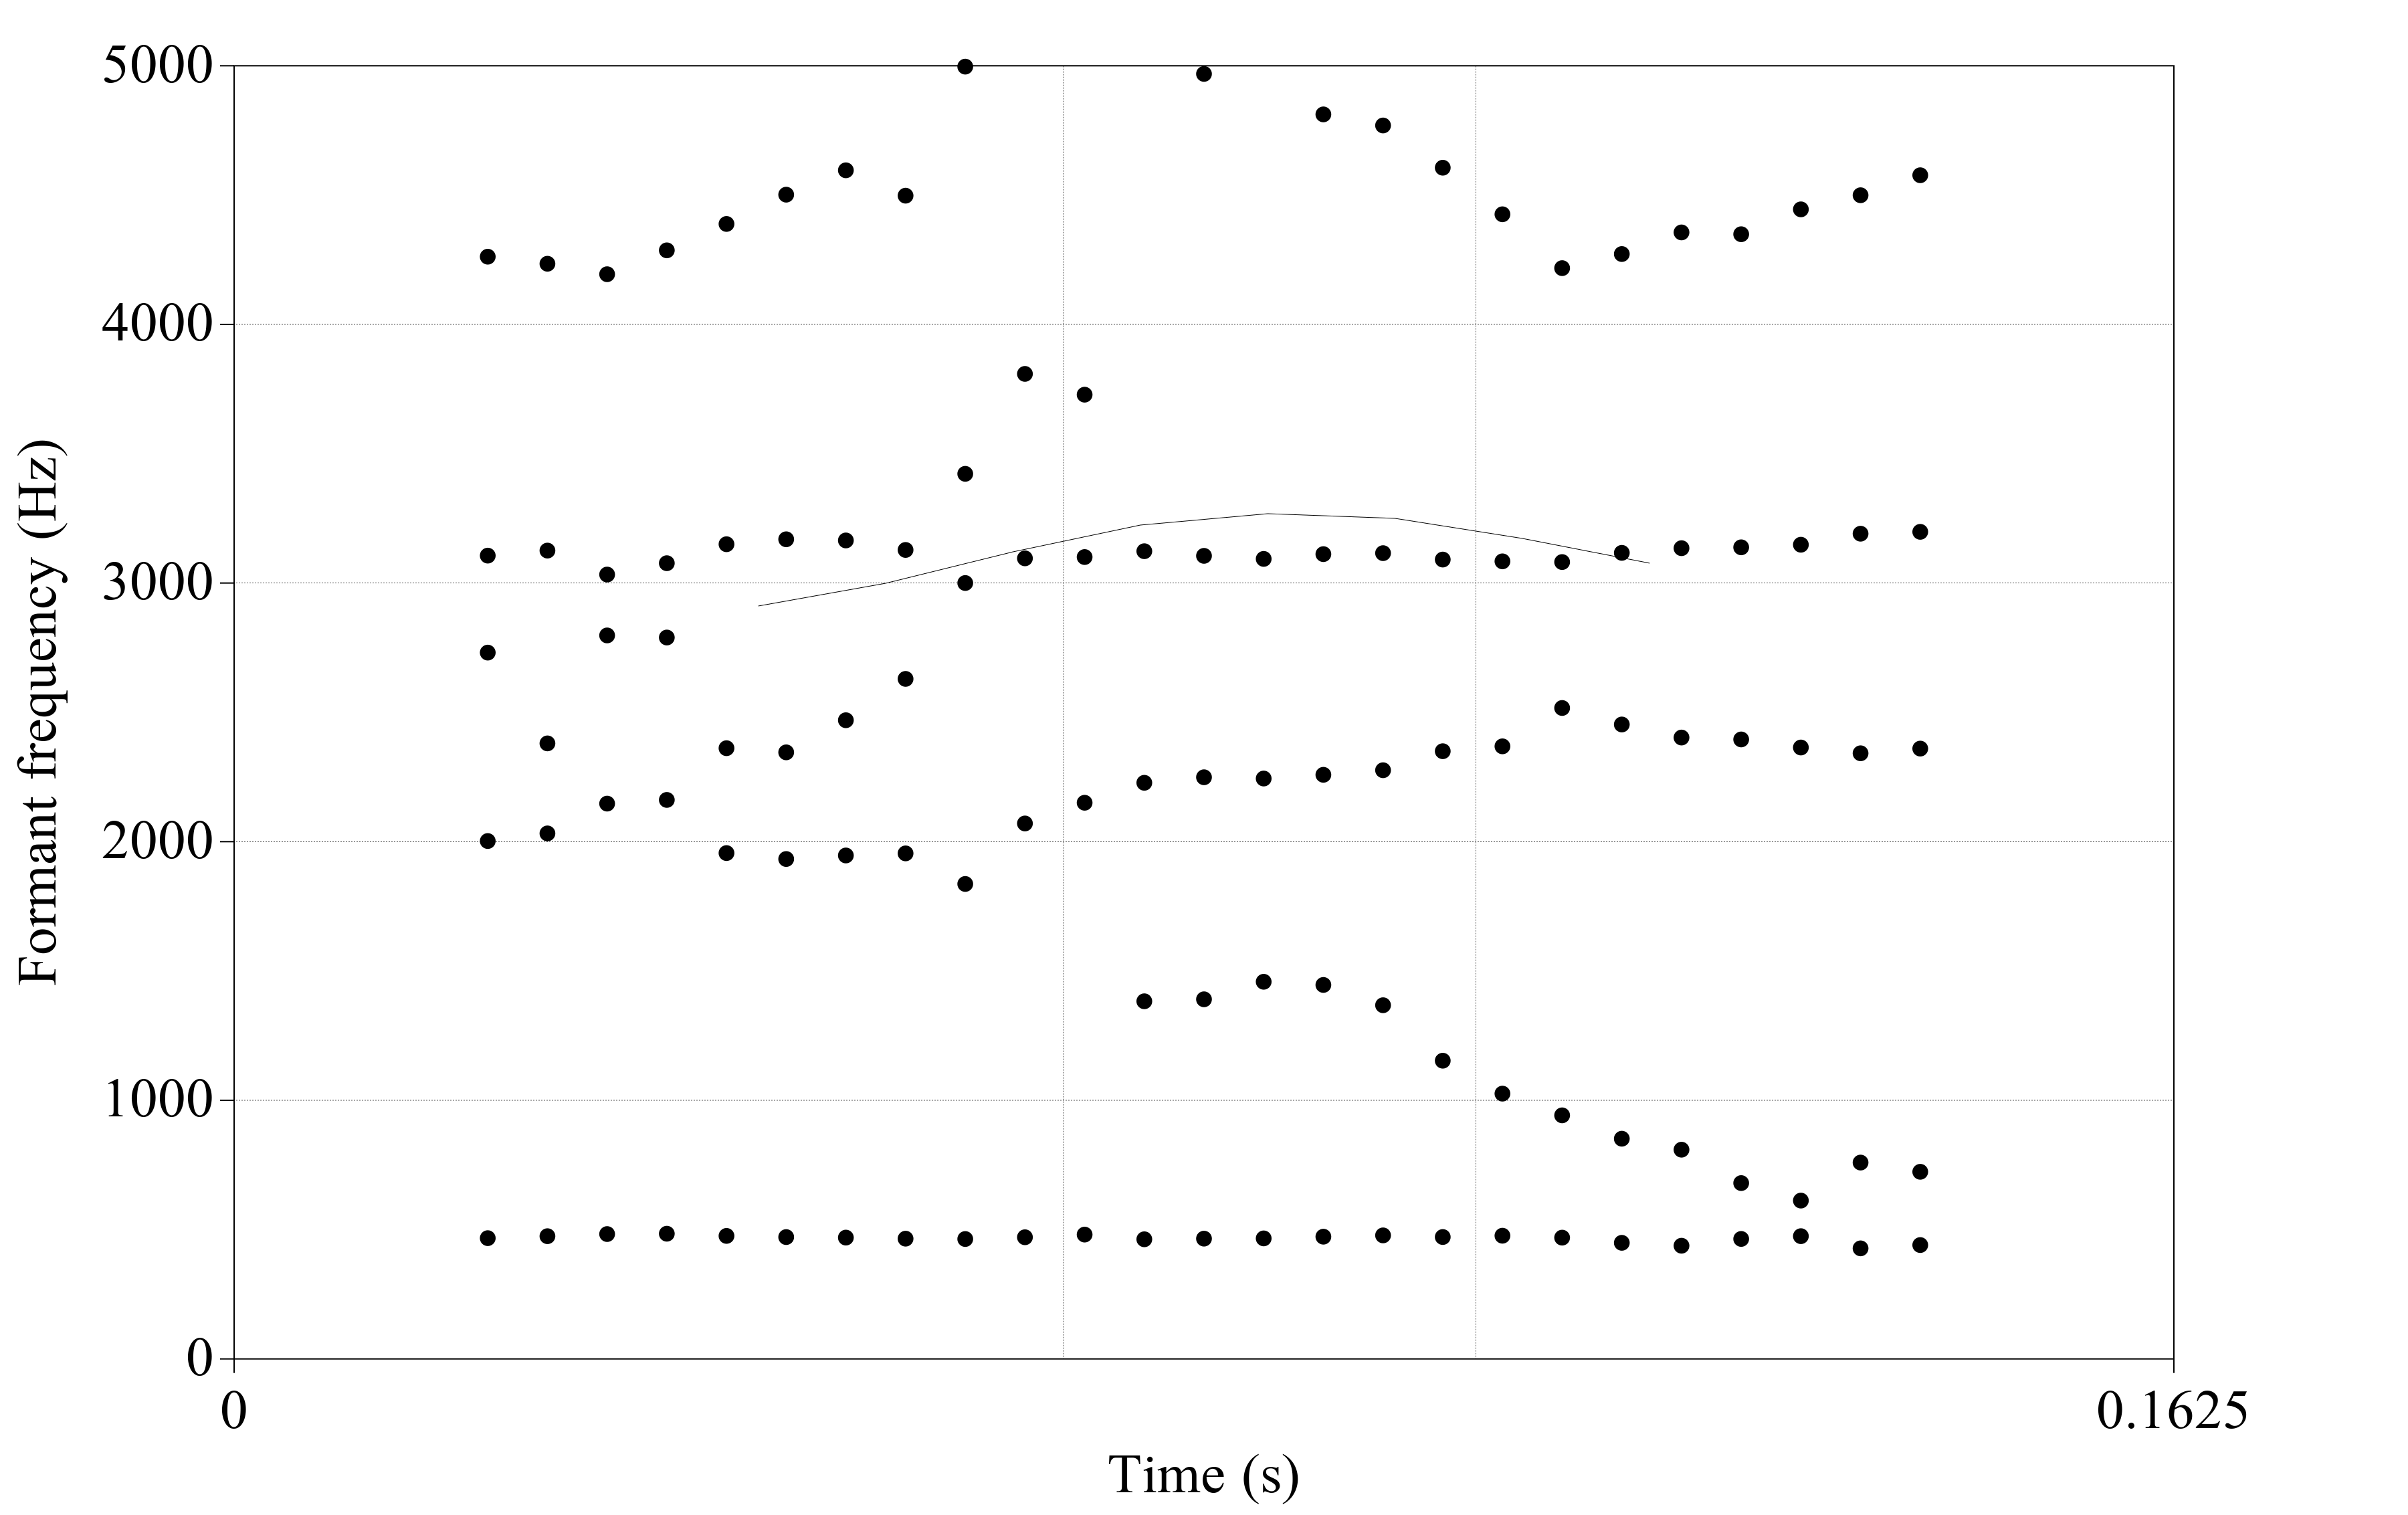
\includegraphics[height = 9.7cm]{images/eu.png}
	\caption{Diptongo /eu/.}
	\label{fig:eu}
\end{figure}

Más allá de los límites de la palabra, la métrica demanda una nueva incursión en el terreno de la fonética porque el diptongo es un mecanismo de ajuste silábico que se da de manera constante en los versos en la unión entre dos palabras cuando la primera acaba en una vocal y la siguiente empieza también con otra. En este caso, una de las dos vocales pierde su calidad vocálica al unirse a la otra. Hablamos aquí de una sinalefa\index{sinalefa}, y el accidente requiere la reevaluación del verso entero, en tanto que afecta al cómputo silábico, como veremos un poco más en detalle más adelante.

Desde una perspectiva acústica, estas propiedades son observables y cuantificables. De acuerdo con \citeauthor{milner2021}~\parencite*{milner2021}, las vocales\index{vocal} puras y los vocoides\index{vocoide} del español presentan diferencias acústicas en su primera y segunda frecuencia fundamental, que son más bajas en las vocales puras. De esta manera, el F2 de \ipa{[i̯]} y \ipa{[u̯]} es más alto que el de \ipa{[i]} y \ipa{[u]}, respectivamente. Se da asimismo una transición entre formantes\index{formante} y amplitud  a lo largo del segmento, lo que acorta la duración del diptongo respecto al hiato. En caso de sinalefa en el verso, se observa de esta manera si el diptongo impropio se realiza como creciente o decreciente.

\begin{table}[!ht]
	\centering\small
	\begin{tabular}{rccccc}
		\toprule
		& \textbf{Tipo} & \textbf{Ejemplo} &\textbf{t. fonológica} & \textbf{t. fonética}\\
		\midrule
		1&/iai/  &	\textit{estudiáis}	&	/estuˈdiais/	&	[estuˈðjai̯s]\\
		2&/iei/  &	\textit{vieira}		&       /ˈvieiɾa/	&	[estuˈðjei̯s]\\
		3&/ioi/  &	\textit{hioides}	&       /ˈioides/	&	[ˈjoi̯ðes]\\
		4&/iau/  &	\textit{«riau»}       &       /riau/		&	[rjau̯]\\
		5&/uai/  &	\textit{averiguáis}       &       /abeɾiˈguais/	&	[abeɾiˈɣwai̯s]\\
		6&/uei/  &	\textit{santigüéis}       &       /santiˈgueis/		&	[santiˈɣwei̯s]\\
		7&/uau/  & 	\textit{guau}       &       /guau/		&	[wau̯]\\
		\bottomrule
	\end{tabular}
	\caption{Triptongos.}
	\label{tab:triptongos
	}
\end{table}


Los triptongos\index{triptongo} son más escasos, y surgen de la combinación de un diptongo creciente y otro decreciente. En español solo hay siete tipos \parencite{canellada1987}. El resultado es un núcleo vocálico precedido de un sonido semiconsonántico y seguido de uno semivocálico. Este núcleo solo lo constituyen los fonemas \ipa{/a/}, \ipa{/e/} y \ipa{/o/}. Los sonidos no vocálicos los forman los fonemas \ipa{/i/} y \ipa{/u/}, con la particularidad de que no se dan las combinaciones \ipa{/ieu/}, \ipa{/iou/}, \ipa{/uoi/}, \ipa{/ueu/} y \ipa{/uou/}. Dicho de otra manera, las siete combinaciones fonéticas posibles son: \ipa{[jai̯]}, \ipa{[jei̯]}, \ipa{[joi̯]}, \ipa{[jau̯]}, \ipa{[wai̯]}, \ipa{[wei̯]} y \ipa{[wau̯]}.

Así pues, la fonología no resulta suficiente por sí misma para caracterizar la sílaba métrica en las uniones vocálicas. Para conocer su naturaleza, es necesario identificar el núcleo y, en caso de secuencia vocálica, localizar qué fonema es el preponderante, ya que los otros son irrelevantes en estas circunstancias.

\subsection{Sonidos consonánticos}\index{consonante}
Aunque no de tanta importancia como las vocales, ya que no afectan a la cuenta silábica, las consonantes desempeñan también un papel esencial. En primer lugar, la consonancia de la rima versal depende de ellas. En segundo, las reglas de división silábica las tienen en cuenta, por lo que su caracterización es necesaria a para deslindar sílabas. Sus propiedades físicas, por otra parte, interesan aquí en tanto que las distinguen de las vocales; las posibles realizaciones alternativas (p.ej. \textipa{/tRans.atˈlan.ti.ko/}, \textipa{/tRan.satˈlan'ti.ko/} o incluso la realización americana \textipa{/tRan.saˈtlan.ti.ko/}) se resuelven mediante reglas, que asumiremos sin entrar en otras discusiones que sobrepasarían el ámbito de este trabajo. Dejamos la puerta abierta a diferentes alternativas en la formalización de estos presupuestos teóricos para adaptar el análisis a un habla particular.

El repertorio del español dispone de tres fonemas oclusivos\index{consonante!oclusiva} sordos con oposición por el punto de articulación. El labial \ipa{/p/}, el dental \ipa{/t/} y el velar \ipa{/k/} \parencite[194-195]{quilis2019}.  De estos fonemas, \ipa{/t/} y \ipa{/d/} tienen realización laminar (predorsal) y \ipa{[t̪]} y \ipa{[d̪]} dentoalveolar \parencite[257]{martinez2003}. A los fonemas sordos se oponen respectivamente los sonoros \ipa{/b/}, \ipa{/d/} y \ipa{/g/}. No obstante, hay que hacer notar que el rasgo oclusivo no es pertinente en las últimas, ya que se realizan por norma general con los alófonos aproximantes \ipa{[β̞]}, \ipa{[ð̞]} y \ipa{[ɣ̞]} \parencite[79-132]{navarrotomas2004}. La realización oclusiva ocurre después de una consonante nasal o de pausa. Asimismo, en el caso de \ipa{/d/}, también se da el alófono oclusivo después de una consonante lateral. Los fonemas \ipa{/k/} y \ipa{/g/} son pospalatales cuando anteceden a \ipa{/i/} o \ipa{/e/}, por lo que su realización es \ipa{[k̞]} y \ipa{[g̞]} o \ipa{[ɣ̞]} \parencite[20-21]{canellada1987}.

Las oposiciones por sonoridad no son pertinentes en posición posnuclear, por lo que la oposición \ipa{/p/}-\ipa{/b/} se neutraliza a /B/ con rasgo común de labialidad, \ipa{/t/}-\ipa{/d/} a /D/ con rasgo común de dentalidad y \ipa{/k/}-\ipa{/g/} a /G/ con rasgo común de velaridad \parencite[205]{quilis2019}.
 
En cuanto a las consonantes nasales\index{consonante!nasal}, todos los fonemas de este tipo en el repertorio español son sonoros. Quilis describe tres fonemas: uno bilabial \ipa{/m/}, otro lingualveolar \ipa{/n/} y uno linguopalatal \ipa{/ɲ/}, que se oponen en posición silábica  prenuclear con una sola realización \ipa{[m]}, \ipa{[n]} y \ipa{[ɲ]} respectivamente \parencite[225]{quilis2019} y se neutralizan en el archifonema\index{archifonema} /N/ en coda. No obstante, \citeauthor{clegg2018}~\parencite*[331-337]{clegg2018} añaden a las realizaciones descritas por Quilis para /m/ la realización alternativa \ipa{[ɱ]} ante una consonante labiodental y para \ipa{/n/}, \ipa{[n̠]} ante un sonido interdental \ipa{[n̪]} ante uno dental, y las palatalizaciones \ipa{[n̠]} ante un sonido palatal y \ipa{[ŋ]} ante uno velar.

\begin{table}[h!]
	\centering\scriptsize
	\begin{tabular}{lcccccccc}
		\toprule	
		\multirow{3}{*}{\shortstack{\textbf{Modo}\\\textbf{de}\\\textbf{articulación}}} & \multicolumn{8}{c}{\textbf{Punto de articulación}} \\
		\cmidrule(lr){2-9}
		& \multicolumn{2}{c}{\textbf{Labial}} & \multicolumn{3}{c}{\textbf{Dental}} & \multirow{2}{*}{\textbf{Palat.}} &  \multicolumn{2}{c}{\textbf{Velar}} \\
		\cmidrule(lr){2-3}\cmidrule(lr){4-6}\cmidrule(lr){8-9}
		& \textbf{Bil.}&\textbf{L.-den.}&\textbf{Den.}&\textbf{Interd.}&\textbf{Alv.}&&\textbf{Vel.}&\textbf{Bil.-alv.}\\
		\midrule
		\textbf{Oclusiva}       &p \quad b&   &t \quad d&   & &   &k \quad g&  \\
		\textbf{Nasal}          &\quad \quad m&\quad \quad [ɱ]&\quad \quad [n̪]&\quad \quad [n̟]&\quad \quad n&\quad \quad ɲ&\quad \quad [ŋ]&  \\
		\textbf{Africada}       &   &   &   &   &   &t͡ʃ\quad[d͡ʒ]&   &  \\
		\textbf{Fricativa}      &   &f \quad \quad& &θ \quad \quad&s\quad\quad&     &x \quad \quad& \\
		\textbf{Aproximante}    &\quad \quad [β̞] &   & &\quad \quad [ð̞]&   &\quad \quad  ʝ [j]&\quad \quad [ɣ̞]&\quad \quad [w]\\
		\textbf{Lateral}        &   &   &\quad \quad [l̪]&\quad \quad [l̟]&\quad \quad l&\quad \quad ʎ&     & \\
		\textbf{Vibrante múlt.} &     &   &   &   &\quad \quad r&      & & \\
		\textbf{Vibrante simp.} &     &   &   &  &\quad \quad ɾ&       & & \\
		\bottomrule
	\end{tabular}
	\caption{Fonemas y alófonos consonánticos del español.}
	\label{tab:consonantes}
\end{table}


Cuando estos tres fonemas están en distensión silábica y preceden a una consonante, incluso entre palabras, su punto de articulación se asimila al de la consonante siguiente. De esta manera, por ejemplo, si la consonante nasal va seguida de una labial, se articula en posición labial (\textlangle{}invento\textrangle{} \ipa{/inˈbento/} \ipa{[imˈbento]}). En tal posición, el punto de articulación deja de ser pertinente y todas las nasales se neutralizan al archifonema /N/ (\ipa{/i\*Nˈbento/}). Este mismo fenómeno sucede en posición final absoluta \parencite[180-182]{alarcos1964}. Estos rasgos han de darse necesariamente porque la neutralización solo se da en fonemas muy cercanos \parencite[228-231]{quilis2019}. Martínez Celdrán \parencite*[51]{martinezceldran2004} hace notar al respecto que \ipa{/ɲ/} no debería considerarse salvo desde una perspectiva diacrónica porque solo se da en posición inicial en español moderno.

El español dispone de cuatro fonemas fricativos\index{consonante!fricativa} \ipa{/f/}, \ipa{/θ/}, \ipa{/s/} y \ipa{/x/} y uno africado\index{consonante!africada} \ipa{/\texttoptiebar{tʃ}/}, así como un sonido aproximante sonoro /ʝ/. Debemos añadir a estos los alófonos aproximantes de /b/, /d/ y /g/ arriba mencionados. Esta colección se refiere al español estándar, pues existen dialectos en los que no se da la oposición entre los fonemas /θ/ y /s/, por lo que optan por /s̄/ en todos los casos, lo que se conoce como \textit{ceceo}\index{ceceo} o por /s/, en cuyo caso hablamos de \textit{seseo}\index{seseo} \parencite[286]{clegg2018}.

El fonema /f/ es labiodental sordo y su realización normal es \ipa{[f]}, que se produce al obstruir el paso del aire colocando los incisivos sobre el labio inferior. Podemos decir que tiene una distribución única con el alófono \ipa{[f]} \parencite[246]{quilis2019}. El fonema  \ipa{/θ/} es interdental o linguinterdental, con el ápice lingual colocado sobre los incisivos \parencite[247]{quilis2019}. Ambos fonemas se sonorizarían ante consonante sonora como \ipa{[v]} y \ipa{[ð]}, respectivamente, aunque, el caso de \ipa{/f/} es muy raro por la escasez de casos de este fonema en posición de coda.

El fonema \ipa{/s/} tiene varias realizaciones para distintos dialectos. En Castilla, la realización es apicoalveolar \parencite[248]{quilis2019}. Este fonema se sonoriza habitualmente ante una consonante sonora y su realización es \ipa{[s̬]} \parencites{torreblanca1978}[251]{quilis2019}, pero puede no ser el caso, especialmente si el hablante  es una mujer \parencite{muniz2012}. Llama la atención que Quilis~\parencite*[251]{quilis2019} indique que el fonema /s/ suele perderse ante \ipa{/r/}, por lo que \textlangle{}dos reales\textrangle{} se pronunciaría \ipa{[ˈdo reˈales]} y, en una pronunciación muy cuidada, con una \ipa{/r/} asibilada [ˈdo ɹeˈales]. \citeauthor{navarrotomas2004}~\parencite*[107]{navarrotomas2004} no va tan lejos y, valiéndose de los mismos ejemplos, propone \ipa{[ˈdos̬ ɹeˈales]}, con una elisión total para casos muy particulares, al igual que hacen \citeauthor{canellada1987}~\parencite*[23]{canellada1987}.

El fonema \ipa{/ʝ/} tiene realización \textit{aproximante}\index{consonante!aproximante} en todos los contextos salvo después de pausa, nasal o lateral, en cuyo caso se presenta como una africada [\ipa{\texttoptiebar{ɟ\textlowering{ʝ}}}] \parencite{martinez2003}. No debe confundirse con el alófono \ipa{[j]} de \ipa{/i/}, que muestra diferencias acústicas y articulatorias significativas. Según \citeauthor{martinezceldran2004}~\parencite*[205-208]{martinezceldran2004}, estas se resumen en que \ipa{[j]} es más breve y con cierta frecuencia apenas un sonido de transición que solo existe acompañado de una vocal nuclear y no se da en ataque sino siempre en posición nuclear, mientras que el sonido \ipa{[\textlowering{ʝ}]} tiene una amplitud menor, de forma especial en $F_{2}$, y solo se da en ataque. A las características de este alófono habría que añadir la explosión con la que comienza el africado \ipa{[\texttoptiebar{ɟ\textlowering{ʝ}}]}. Tampoco debe confundirse con el sonido lateral \ipa{/ʎ/} \parencite[287]{clegg2018}, presente en el habla cuidada.

El fonema /x/ es velar en el español de Castilla, con un alófono \ipa{[χ]} antes de \ipa{/o/} y \ipa{/u/} en todas sus realizaciones \parencite{martinez2003}. Por su parte, el africado \ipa{/\texttoptiebar{tʃ}/} es linguopalatal sordo.

En lo que respecta a las \textit{consonantes líquidas}\index{consonante!líquida}, encontramos dos laterales con sus respectivos alófonos y dos vibrantes, una simple y otra múltiple. Las laterales\index{consonante!lateral} en español son \ipa{/l/} y \ipa{/ʎ/}, aunque esta última está en vías de desaparición y predomina únicamente en las variedades septentrionales ibéricas y en las tierras altas americanas, siendo lo habitual en el sur de España y América que se neutralice a /ʝ/. Las laterales se caracterizan por presentar formantes\index{formante} atenuados debido al cierre central, que, junto a las transiciones vocálicas —menos abruptas, en cualquier caso, que para las consonantes nasales—, indican el lugar de articulación.

El fonema /l/ es lateral lingualveolar y se realiza como \ipa{[l]}, salvo en algunas posiciones silábica posnucleares \parencite[309-310]{quilis2019}. Cuando precede a \textipa{/T/}, se desplaza hasta una posición interdental (\textlangle{}colza\textrangle{} \textipa{[ko\textsubplus{l}Ta]}), antes de \ipa{/t/} o \ipa{/d/} es linguodental (\textlangle{}caldo\textrangle{} \textipa{[ka\textsubbridge{l}do]}) y ante palatal se realiza linguopalatalizado (\textlangle{}el ñu\textrangle{} \textipa{[e\textsubbar{l} \textltailn u]}) \parencite[341-250]{clegg2018}. El fonema \ipa{/l/} se da en la posición inmediatamente anterior o posterior al núcleo vocálico, mientras que \textipa{/ʎ/} solo aparece en posición prenuclear en palabras patrimoniales. Esto hace cuestionable una neutralización a /L/ de las laterales desde una perspectiva sincrónica.

En castellano encontramos una consonante vibrante\index{consonante!vibrante} simple\index{consonante!vibrante!simple} \textipa{/R/} y una múltiple\index{consonante!vibrante!múltiple} \ipa{/r/}. Se producen colocando el ápice de la lengua contra los alvéolos para generar una o varias oclusiones. Ambas son apicoalveolares y no tienen más que un alófono. La vibrante simple solo aparece en interior de palabra en posición prenuclear entre vocales (\textlangle{}hora\textrangle{} \textipa{/ˈoRa/}) o entre \ipa{/p/}, \ipa{/t/}, \ipa{/k/}, \ipa{/b/}, \ipa{/d/}, \ipa{/g/} o \ipa{/f/} y vocal (\textlangle{}protráctil\textrangle{} \textipa{/pRoˈtRaktil/}, \textlangle{}crabrón\textrangle{} \textipa{/kRaˈbRon/} y \textlangle{}grecofrancés\textrangle{} \textipa{/gRekofRanˈTes/} ) \parencite[330]{quilis2019}. La oposición  entre \ipa{/r/} y \textipa{/R/}  solo es pertinente fonológicamente en posición intervocálica (\textlangle{}perro\textrangle{} \ipa{/pero/}-\textlangle{}pero\textrangle{} \textipa{/peRo/}), por lo que en todas las demás posiciones se neutraliza al archifonema /R/ \parencite{alarcos1964}.

Al contrario que con las vocales, la caracterización fina de las consonantes sí tiene consecuencias en el metro. Dicho de forma más precisa, la neutralización fonémica podría afectar a una parte tan importante como es la rima. Si bien resultaría difícil hallarlo, es una posibilidad teórica real. Por ejemplo, \textlangle{}Abraham\textrangle{} y \textlangle{}Guzmán\textrangle{} serían \textipa{/abraˈa}N/ y \textipa{/guTˈma}N/ y, por lo tanto, formarían rima consonante.

\section{División silábica del español}\label{sec:silabas}
\subsection{Características generales}
La sílaba española consiste en un núcleo vocálico obligatorio, opcionalmente precedido de un ataque o seguido de una coda, ambos consonánticos (\Cref{fig:silabeo}). El núcleo consta generalmente de una sola vocal como /o/ en \textlangle{}ocaso\textrangle{} \ipa{[o.ˈka.so]}, pero puede ir unido a vocales débiles en forma de vocoide\index{vocoide}, precedido de una semiconsonante como en \textlangle{}idiota\textrangle{} \ipa{[i.ˈðjo.ta]}\index{semiconsonante} o seguido de una semivocal\index{semivocal} como en \textlangle{}hoy\textrangle{} \ipa{[oi̯]}, lo que constituiría sendos diptongos, o incluso orlado a ambos lados, como en \textlangle{}dioico\textrangle{} \ipa{[ˈðjoi̯.ko]}, en cuyo caso hablaríamos de triptongo\index{triptongo}. Por su parte, tanto coda como ataque, cuando se dan, están compuestos por entre una y dos consonantes. Se denomina sílaba libre a aquella que consta de un núcleo vocálico en solitario o acompañado de uno o dos sonidos consonánticos en ataque, y trabada a la que tiene más de un sonido consonántico en coda \parencite[46-47]{navarrotomas1946}.

\begin{figure}[!ht]
	\centering
\begin{tikzpicture}
\tikzset{frontier/.style={distance from root=150pt}}
    \Tree   [.{\textbf{Palabra}} 
[.{\textbf{\upshape S$_1$}} 
[[.\textit{Ataque} [.C$_1$ {\textit{t}} ] 
[.C$_2$ {\textit{r}} ]]] 
[.\textit{Rima}
[.\textit{Núcleo} [.C$_1$ {\textit{a}} ] ]
[.\textit{Coda}  [.C$_2$ {\textit{n}} ] 
[.C$_2$ {\textit{s}} ] ] ] ]
%
%
[.{\textbf{\upshape S$_2$}} 
[[.\textit{Ataque} [.C$_1$ {\textit{p}} ]] ]
[.\textit{Rima}
[.\textit{Núcleo}  [.S$_1$ {\textit{u}} ]
[.V {\textit{e}} ] ]
[.\textit{Coda} [.C$_1$ {\textit{s}} ] ]]]
%
%
[.{\textbf{\upshape S$_3$}} 
[[.\textit{Ataque} [.C$_1$ {\textit{t}} ] ]]
[.\textit{Rima}
[.\textit{Núcleo}  [.V {\textit{o}} ] ]]]
]
\end{tikzpicture}

\caption{Construcción sílabas.}
\label{fig:silabeo}
\end{figure}

De acuerdo esto, tenemos nueve combinaciones posibles del núcleo con hasta dos consonantes en ataque o en coda, distribuidas según lo mostrado en el ejemplo \ref{ex:silabaaa}. 
\begin{exe}\ex\label{ex:silabaaa}
\begin{tabular}{ l l }
	V & \textit{y}, \textit{o},  \\ 
	CV & \textit{la}, \textit{de},  \\
	VC & \textit{un}, \textit{él}  \\ 
	CVC & \textit{mar}, \textit{ven}, \\ 
	CCV & \textit{\textbf{bra}·sa}, \textit{la·\textbf{cre}}  \\
	VCC & \textit{\textbf{obs}·ce·no},  \textit{\textbf{ins}·pi·ra·ción} \\
	CCVC & \textit{\textbf{bron}·ce}, \textit{im-\textbf{pren}·ta} \\ 
	CVCC & \textit{\textbf{pers}·pec·ti·va}, \textit{\textbf{cons}·cien·te}  \\ 
	CCVCC & \textit{\textbf{trans}·mu·tar}
\end{tabular}
\end{exe}
Cualquier consonante puede ocupar la posición de ataque en solitario. Sin embargo, si hay dos consonantes, no todas las combinaciones son posibles. En posición de coda ocurre lo mismo, con la restricción adicional de que determinadas consonantes no se dan jamás en dicha posición.

Asimismo, aparece como máximo una sola consonante a final de palabra en español moderno, al contrario que en otras variedades diacrónicas donde se dan casos como \textit{puent}, \textit{muert} \parencite[49]{navarrotomas1946}. No obstante, las pocas coincidencias relativamente recientes que se encuentran en el CORDE  nos remiten a documentos de la primera mitad del siglo \textsc{xvi}, por lo que, considerando asimismo que el registro escrito es más conservador que la lengua hablada, asumimos que el español del Siglo de Oro se comporta en este sentido como la variedad moderna.

\subsection{División entre vocales}\label{sec:irregularidades}
En la división vocálica podemos distinguir los casos vocal\textsuperscript{$+\textsc{alta}$} vocal\textsuperscript{$+\textsc{alta}$}, vocal\textsuperscript{$+\textsc{alta}$} vocal\textsuperscript{$-\textsc{alta}$}, vocal\textsuperscript{$-\textsc{alta}$} vocal\textsuperscript{$+\textsc{alta}$} y vocal\textsuperscript{$-\textsc{alta}$} vocal\textsuperscript{$-\textsc{alta}$}. Exclusivamente el último de los cuatro casos forma siempre un hiato. Todos los otros casos constituyen diptongo o hiato \parencite{riosmestre1999}. De esta forma, \textlangle{}crear\textrangle{} será necesariamente bisilábica \textipa{/kReˈaR/}, pero tenemos \textlangle{}lío\textrangle{} \textipa{/ˈli.o/} \ipa{[ˈli.o]},
\textlangle{}lio\textrangle{} \textipa{/liˈo/} \ipa{[liˈo]} o \textlangle{}vio\textrangle{} \ipa{/bio/} \ipa{[Bjo]} 
y \textlangle{}voy\textrangle{} \textipa{/ai/} \ipa{[ai̯]} o \textlangle{}ahí\textrangle{} \ipa{/a.ˈi/} \ipa{[a.ˈi]}, y \textlangle{}fui\textrangle{} \ipa{/fui/} \ipa{[fwi]} o \textlangle{}hui\textrangle{} \ipa{/u.ˈi/} \ipa{[/u.ˈi/]}. Aunque la división silábica se infiere de la ortografía la mayoría de las veces, este no es siempre el caso, como vemos, por ejemplo, en \textlangle{}criado\textrangle{} \textipa{/kRi.ˈa.do/} \textipa{[kRi.ˈa.ðo]} y \textlangle{}aciago\textrangle{} \textipa{/a.ˈTia.go/} \textipa{[a.ˈTja.Go]}.

De acuerdo con \citeauthor{quilis2019}~\parencite*[184-186]{quilis2019}, dos vocales átonas forman diptongo si al menos una de ellas es alta. La secuencia vocal\textsuperscript{$+\textsc{alta}$} vocal\textsuperscript{$-\textsc{alta}$} o vocal\textsuperscript{$-\textsc{alta}$} vocal\textsuperscript{$+\textsc{alta}$} forma diptongo cuando la vocal alta es tónica. El resto de los casos suele formar diptongo, salvo en los siguientes casos descritos por el autor:

\paragraph{Verbos en \textit{-iar}:}{\textit{agriar}, \textit{aliar}, \textit{ampliar}, \textit{arriar}, \textit{ataviar}, \textit{autoviar}, \textit{aviar}, \textit{ciar}, \textit{confiar}, \textit{congloriar}, \textit{contrariar}, \textit{criar}, \textit{desafiar}, \textit{desaviar}, \textit{descarriar}, \textit{desconfiar}, \textit{desvariar}, \textit{desviar}, \textit{enfriar}, \textit{enviar}, \textit{espiar}, \textit{estriar}, \textit{expiar},  \textit{extraviar}, \textit{ferroviar}, \textit{fiar}, \textit{gloriar}, \textit{grafiar}, \textit{guiar}, \textit{hastiar}, \textit{istriar}, \textit{liar}, \textit{malcriar}, \textit{piar}, \textit{porfiar}, \textit{recriar}, \textit{reenviar}, \textit{resfriar}, \textit{triar} y \textit{vaciar}. Previene, no obstante, que no afecta el futuro y al condicional porque, mientras que en \textit{fiar}, \textit{fía} o \textit{fio} una de las vocales es tónica, en \textit{fiaré} o \textit{fiaría} son ambas átonas.}

\paragraph{Verbos en \textit{-uar}:}{\textit{acentuar}, \textit{actuar}, \textit{atenuar}, \textit{cansuar}, \textit{conceptuar}, \textit{contextuar}, \textit{continuar}, \textit{descontinuar}, \textit{desgraduar}, \textit{deshabituar}, \textit{desvirtuar}, \textit{estatuar}, \textit{evaluar}, \textit{exceptuar}, \textit{extenuar}, \textit{fluctuar}, \textit{ganzuar}, \textit{graduar}, \textit{habituar}, \textit{individuar}, \textit{infatuar}, \textit{insinuar}, \textit{menstruar}, \textit{perceptuar}, \textit{perpetuar}, \textit{puar}, \textit{puntuar}, \textit{ruar}, \textit{situar}, \textit{tatuar}, \textit{tumultuar},  \textit{usufructuar} y \textit{valuar}, y se exceptúan los verbos terminados en \textit{-cuar} \textipa{[kwaR]} y \textit{-guar} \textipa{[gwaR]}, que forman diptongo en todos los casos y, por el mismo motivo que los verbos en \textit{-iar}, el futuro y el condicional.}
	
\paragraph{Verbos en \textit{-uir}:}{\textit{afluir}, \textit{argüir}, \textit{atribuir}, \textit{circuir}, \textit{concluir}, \textit{constituir}, \textit{construir}, \textit{contribuir}, \textit{derruir}, \textit{destituir}, \textit{destruir}, \textit{diluir}, \textit{disminuir}, \textit{distribuir}, \textit{esmuir}, \textit{estatuir}, \textit{excluir}, \textit{fluir}, \textit{huir}, \textit{imbuir}, \textit{incluir}, \textit{influir}, \textit{inmiscuir}, \textit{instituir}, \textit{instruir}, \textit{intuir}, \textit{irruir}, \textit{muir}, \textit{obstruir}, \textit{ocluir}, \textit{prostituir}, \textit{recluir}, \textit{reconstituir}, \textit{reconstruir}, \textit{redargüir}, \textit{refluir}, \textit{rehuir}, \textit{restituir}, \textit{retribuir} y \textit{sustituir}. La excepción del condicional y el futuro aplica aquí también.}

\paragraph{Adjetivos en \textit{-uoso(s)}/\textit{-uosa(s)}:}{\textit{suntuoso}, \textit{virtuoso}, \textit{sinuoso}}.

\paragraph{Casos particulares y sus flexiones:}{\textit{acuoso}, \textit{anual},  \textit{arriero}, \textit{bienio}, \textit{biombo}, \textit{boquiancho}, \textit{cliente}, \textit{crianza}, \textit{cruel}, \textit{desconfianza}, \textit{diablo}, \textit{diálogo}, \textit{dieciocho}, \textit{ferrovial}, \textit{fianza}, \textit{gorrión}, \textit{guión}, \textit{hiato}, \textit{maniobra}, \textit{miasma}, \textit{piano}, \textit{prior}, \textit{santuario}, \textit{Sión}, \textit{tiara}, \textit{triángulo}, \textit{trienio}, \textit{truhán} y \textit{ventiocho}. Navarro~Tomás~\parencite*[68]{navarrotomas2004} añade \textit{ruido}, \textit{suave}, \textit{viaje} y \textit{viuda}.}

\paragraph{Secuencias /ˈi.u/, /ˈu.i/, /iˈu/ o /uˈi/:}{\textit{jesuita}, \textit{circuito}, \textit{fortuito}, \textit{casuística} y \textit{diurno}.}

A esto debemos añadir los verbos en \textit{-eír} \parencite[6.8.2.1.2.2]{riosmestre1999}, como \textit{desleír}, \textit{engreír}, \textit{freír}, \textit{refreír}, \textit{reír}, \textit{sofreír} y \textit{sonreír}. Se volvería a excluir el futuro y el condicional. \citeauthor{riosmestre1999}~\parencite*[6.8.2.1.2.3]{riosmestre1999} alude asimismo a los verbos en \textit{-oír}, pues considera inoportunas las salvedades del futuro y el condicional. 

\citeauthor{canellada1987}~\parencite*[51-52]{canellada1987} señalan asimismo \textit{ahilarse}, \textit{baulero}, \textit{buhonero}, \textit{criador}, \textit{huidizo}, \textit{miopía}, \textit{prohibir}, \textit{reunión}, \textit{reiré} y \textit{semiesfera}. Observamos que estos son bien derivados de palabras sin ambigüedad ortográfica, de las excepciones descritas o resultado de la prefijación, a excepción de \textit{buhonero}, \textit{miopía} y \textit{prohibir}.

No hemos considerado prefijos acabados en vocal como \textit{re-} o \textit{tri-} (por ejemplo, \textit{rehilamiento} y \textit{triángulo}), que podrían tender a formar hiato en algunas circunstancias, como un habla muy lenta, dado que la literatura al respecto ha resultado ser muy escasa. Sin embargo, incluimos un archivo de excepciones en la formalización donde forzar el hiato en casos particulares para modificar el comportamiento del módulo que realiza la silabación. Las entradas correspondientes llevan una marca que las identifica como comentarios y no como reglas, por lo que no se tienen en cuenta; esta marca se borra discrecionalmente cuando se desea hacer el hiato.

\subsection{División entre consonantes}
Podemos distinguir los siguientes casos: una consonante intervocálica, grupo de dos consonantes intervocálicas, tres o más consonantes intervocálicas, que Quilis~\parencite*[367-369]{quilis2019} resuelve de tres maneras diferentes.

\paragraph{V-C-C-V:}{El caso más simple es el de una consonante intervocálica. Dado que el español tiene tendencia a las sílabas abiertas, dicha consonante se agrupará con la sílaba siguiente.}


\paragraph{V-C-C-V:}{Si las consonantes son una agrupación de consonante del tipo \textit{muta cum liquida}, esto es bilabial o labiodental (/p/, /b/, /f/) o linguovelar (/g/, /k/) seguida de una líquida (\textipa{/R/}, /l/) o una linguodental(/d/, /t/) seguida de vibrante (\textipa{/R/}), nos encontramos ante una unidad inseparable que forma la coda del núcleo silábico siguiente (\textit{probar}, \textit{plomo}, \textit{broma}, \textit{blanco}, \textit{francés}, \textit{flanco},\textit{gracia}, \textit{glosa}, \textit{craso},  \textit{claro},  \textit{drama},  \textit{trama}). Cualquier otra combinación se reparte entre la primera y la segunda sílaba.}

\paragraph{V-C-C-C-(C)-V:}{Para que se dé una combinación de tres consonantes, los dos últimos fonemas deben formar una unidad inseparable como las descritas en el párrafo anterior o bien las dos primeras deben ser una agrupación del tipo /Ns/ o /Bs/ (\textlangle{}constar\textrangle{} \textipa{/konsˈtaR/}, \textlangle{}obstar\textrangle{} \textipa{/obsˈtaR/}). Si hay cuatro consonantes seguidas se trata de una conjunción de ambos casos (\textlangle{}abstracción\textrangle{} \textipa{/abs.tRakˈTion/}), por lo que se reparten dos en cada núcleo.}

\subsection{Contacto entre vocales de diferentes palabras}
El principio fundamental de la reducción vocálica a grupos silábicos reza que, según la fonética, dos vocales cualesquiera en contacto admiten reducirse siempre a una sola sílaba, por lo que lo harán si no hay razones gramaticales o de otra índole que lo impidan \parencite[136]{navarrotomas2004}. \citeauthor{canellada1987}~\parencite*[55]{canellada1987} hacen una descripción detallada de las circunstancias que concurren en los límites de palabra cuando hay dos vocales en contacto y cómo se resuelven estas uniones. Según los autores, se producen cuatro tipos de unión: \textit{hiato}\index{hiato}, \textit{reducción}\index{reducción}, \textit{diptongación}\index{diptongo} y \textit{elisión}\index{elisión}. Salvo en el hiato, hablaremos en estos casos de \textit{sinalefa}. Llamamos sinalefa\index{sinalefa} a la unión en una única sílaba de dos vocales adyacentes ubicadas en posición final e inicial de sendas palabras contiguas. Pueden unirse de esta manera hasta cinco vocales distribuidas a lo largo de hasta tres palabras, como, por ejemplo, en \textlangle{}repudio a Eugenia\textrangle{} \ipa{[reˈpu.djo̯ae̯u̯ˈxe.nja]}. Para que ocurra una sinalefa han de cumplirse cuatro condiciones:
\begin{enumerate}
	\item La pronunciación debe ser rápida.
	\item No hay enfatizaciones.
	\item Si intervienen más de dos vocales, entre dos vocales abiertas solamente puede haber otra abierta.
\end{enumerate}

Si no se cumplen estas condiciones, lo normal es que se produzca un hiato \textipa{/boi̯.aˈka.sa/} o, si acaso, que se redistribuyan las fronteras silábicas \textipa{/bo.Jaˈka.sa/}. Cuando sí concurren todas las condiciones necesarias, la resolución de la sinalefa varía en función de las partes que la constituyen. 

De esta manera, si  se encuentran dos vocales iguales, estas se funden en una. Si el resultado tiene más cantidad, hablaríamos de reducción\index{reducción} (\ref{ex:red}). Por el contrario, si la cantidad es regular, hablaremos de elisión\index{elisión} (\ref{ex:eli}). La realización según uno u otro recurso depende sobre todo de la velocidad de la pronunciación. Además, si una de las vocales es tónica, la unión también será tónica \parencite[138-139]{navarrotomas2004}.
\begin{exe}
\ex\textlangle{}va a verlo\textrangle{}\begin{xlist}
\ex{\textipa{/ˈba:ˈbeR.lo/}}\label{ex:red}
\ex{\textipa{/ˈbaˈbeR.lo/}}\label{ex:eli}	
\end{xlist}
\end{exe}

Si las vocales son diferentes, una de las dos pierde su condición silábica, pero conservar el timbre vocálico. En este caso, se trataría de una reducción  (\ref{ex:red1}). Cuál de ambas vocales hace de núcleo y cuál se reduce depende de varios factores. Si ambas son átonas, el elemento de la segunda posición tiene precedencia (\ref{ex:red2}). Si una de las dos partes es tónica y la otra no, se prefiere la vocal tónica para hacer de núcleo (\ref{ex:red3}). En cualquier otro caso, la vocal más abierta precede a la más cerrada como posible núcleo (\ref{ex:red4}) \parencite[140-152]{navarrotomas2004}.
\begin{exe}
	\ex\label{ex:red1}\textlangle{}se acerca\textrangle{} \textipa{/se̯aˈTeR.ka/}
		\ex\label{ex:red2}\textlangle{}parece huraño\textrangle{} \textipa{/paˈRe.Te̯uˈRa.No/}
		\ex\label{ex:red3}\textlangle{}la hebra\textrangle{} \textipa{/ˈla̯e.bRa/}/
		\ex\label{ex:red4}\textlangle{}va este\textrangle{} \textipa{/ˈbae̯s.te/}
\end{exe}
En el último caso, hay que tener además en cuenta la escala de perceptibilidad, que, según \citeauthor{navarrotomas2004}~\parencite*[25]{navarrotomas2004}, se establece según el grado de apertura bucal, por lo que /a/ sería la vocal más perceptible, seguida de /o/ y de /e/ y las menos perceptibles serían /i/ y /u/. Asimismo, al igual que ocurre entre vocales iguales, si una de las partes de la unión es tónica, la sílaba resultante también lo será \parencite*[142]{navarrotomas2004}.

Si la vocal que pierde su calidad de núcleo silábico es /i/ o /u/, también lo hace con su condición vocálica, de forma que \textlangle{}mi amigo\textrangle{} se pronunciaría \textipa{/mjaˈmi.go/} en ese caso. Además, si la vocal cerrada es tónica, el acento se desplaza a la siguiente vocal. Esto es, en \textlangle{}salí ayer\textrangle{} \textipa{/saˈljaˈJeR/}, el acento recaería en \ipa{[a]}. Esto se confirma también en la poesía \parencite{esgueva2004}.

La elisión total, aunque no es ajena a la lengua hablada —especialmente en expresiones hechas como \textit{*sabusté} o \textit{*sacabao}—, se considera propia de registros vulgares. En cualquier caso, dado que, en las representaciones dramáticas de las que nos ocupamos, el habla es intencionalmente cuidada —se declama—, esta situación no debería suponer un inconveniente. Podemos asumir que el dramaturgo habría indicado explícitamente si alguna pronunciación ha de ser deliberadamente inadecuada, como, por ejemplo, cuando un rústico habla sayagués. Aquí, claro está, se hace patente la necesidad de una buena edición que enmiende el exceso de celo corrector de algún cajista. 

Si la agrupación es de más de dos vocales, la reducción no es siempre posible. Para que esto suceda, deben estar agrupadas de menor a mayor perceptibilidad si la última vocal es nuclear (\ref{ex:menosmas}), y viceversa si es la primera (\ref{ex:masmenos}). Si la vocal nuclear ocupa una posición central, el grado de perceptibilidad de las vocales no nucleares debe reducirse en ambas direcciones  (\ref{ex:menosmasmenos}), de modo que, si la secuencia vocálica continúa, la vocal menos perceptible represente la división silábica.

\begin{exe}
	\ex\label{ex:menosmas}\textlangle{}espíritu o aliento\textrangle{} \textipa{/esˈpi.Ri.tu̯o̯aˈljen.to/}
	\ex\label{ex:masmenos}\textlangle{}halla o ubica\textrangle{} \textipa{/ˈa.Lao̯u̯ˈbi.ka/}
	\ex\label{ex:menosmasmenos}\textlangle{}vengo a esperar\textrangle{} \textipa{/ˈven.go̯ae̯s.peˈRaR/}
\end{exe}

Puede darse en este último caso la ambigüedad de que la vocal reducida liminar se agrupe indistintamente con el primer núcleo (\ref{ex:menosmasmenosmasa}) o con el segundo (\ref{ex:menosmasmenosmasb}).
\begin{exe}
	\ex\textlangle{}la he asado\textrangle{}
	\begin{xlist}
		\ex\label{ex:menosmasmenosmasa}\textipa{/ˈla̯e.aˈsa.do/}
		\ex\label{ex:menosmasmenosmasb}\textipa{/laˈe̯aˈsa.do/}
	\end{xlist}
\end{exe}

\subsection{Conjunciones \textit{y}/\textit{e} y \textit{o}/\textit{u}}\index{conjunción}\label{sec:conj}
La conjunción \textit{y} se une a las siguientes vocales observando unas normas \parencites[59]{canellada1987}[49]{navarrotomas2004}. Cuando aparece en posición interconsonántica, se pronuncia como \ipa{/i/} de relajación variable. Cuando va entre una consonante y una vocal, se realiza como semiconsonante en diptongo con el fonema vocálico siguiente y se pronuncia \ipa{/j/}, salvo que vaya precedida de \ipa{/s/} o \ipa{/z/}, en cuyo caso la pronunciación será consonántica y se unirá en ataque como \ipa{/ʝ/}. En la situación inversa, si va precedido de una vocal y seguido de una consonante, diptonga con el núcleo vocálico precedente en calidad de semivocal como \ipa{/i̯/}. La última posibilidad es que se encuentre entre dos vocales, en cuyo caso tendrá calidad consonántica y se unirá en ataque a la sílaba de su derecha como \ipa{/ʝ/}.

Las conjunciones \textit{e}, \textit{o} y \textit{u} suelen unirse con una consonante final de la primera palabra y diptongan con la vocal inicial de la segunda \parencite[60]{canellada1987}. Entre vocales, suele producirse un hiato con la primera palabra y un diptongo con la segunda tanto para \textit{e} como para \textit{o} \parencite[60]{canellada1987}. Lo mismo señala \citeauthor{bello1981}~\parencite*[109-111]{bello1981}, que llama la atención sobre lo áspera que se hace al oído castellano la ligadura de dos vocales por \textit{o}. No obstante, Bello indica que la conjunción \textit{e} funciona de manera opuesta, uniéndose a la vocal precedente. 
	
\section{Transcripción grafémico-fonológica}\label{transgraffon}
\citeauthor{riosmestre1999}~\parencite*[2.3]{riosmestre1999} describe tres procedimientos de transcripción: por reglas\index{transcripción!por reglas}, si se toma como entrada los grafemas\index{grafema} para transformarlos, por diccionario\index{transcripción!por diccionario}, si se toman unidades léxicas, y la pronunciación por analogía, basada en la inteligencia artificial. Los sistemas basados en reglas son los menos costosos de construir porque se fundamentan en la sistematización de la teoría lingüística. Estos se modifican de manera sencilla y la corrección de errores es rápida. Como contrapartida, son lentos, y su velocidad disminuye en función del número de reglas por lo que, a mayor precisión, mayor lentitud. La transcripción por diccionarios es más exacta además de veloz, pero, por su propia naturaleza, solo admite transcribir palabras previamente almacenadas. Independientemente de esto, decidirse por uno u otro método requiere, además, tener en cuenta otro aspecto fundamental: la relación entre grafema\index{grafema} y fonema\index{fonema} de la lengua en cuestión. 

El sistema de reglas se ha empleado tradicionalmente en la conversión de texto a habla, con buenos resultados \parencites{perez1991}{lopez1993}{rodriguez1998}, pero no siempre conduce a una resolución óptima de todos los casos si la ortografía no da lugar a la interpretación fonética libre de ambigüedad. En esos casos, las irregularidades demandan procedimientos específicos. Entre estos, señalaremos  la regularización de las excepciones ortográficas o las listas de palabras \parencite*[2.3]{riosmestre1999}. Esta última aproximación usaría la transcripción mediante diccionario como apoyo para la transcripción por reglas.

En cuanto a la formalización de las reglas, \citeauthor{riosmestre1999}~\parencite*[2.4]{riosmestre1999} se basa en \citeauthor{chomsky1968}~\parencite*{chomsky1968} para enunciar cuatro tipos de reglas de transformación. Primero, habría reglas biunívocas, cuando un grafema se transcribe con un único fonema, por ejemplo, \textlangle{}t\textrangle{} $\rightarrow$ /t/. El siguiente tipo sería la correspondencia dos a uno, en el caso de un dígrafo\index{dígrafo}, por ejemplo \textlangle{}qu\textrangle{} $\rightarrow$ /k/. También se da el caso contrario, con una correspondencia uno a dos, cuando a un grafema le corresponden dos fonemas, como en el caso de  \textlangle{}x\textrangle{} $\rightarrow$ /ks/. Finalmente, existe la posibilidad de una correspondencia uno a cero, cuando a un grafema\index{grafema}, como \textlangle{}h\textrangle{}, no le corresponde fonema alguno.

Las reglas simples de reescritura pueden formar un sistema booleano complejo, con la derivación mediante operaciones unarias como la negación, o binarias como la combinación de dos reglas entre sí. Estas, a su vez, se aplican de forma recursiva. Asimismo, resulta conveniente bajo ciertas circunstancias valerse de definiciones, en lugar de secuencias y reglas \textit{globales}, que consideren estados anteriores de la derivación \parencite[2.4]{riosmestre1999}

De acuerdo con la descripción de \citeauthor{vanleuwen1989}~\parencite*{vanleuwen1989}, tenemos un texto de entrada y uno de salida. El primero es grafémico y el segundo es su transcripción fonética. A los caracteres de estos textos los denominamos \textit{segmentos}, y la herramienta para operar en ellos es la regla lingüística. Cada segmento se traducirá conforme a su contexto según la forma propuesta por \citeauthor{chomsky1968}~\parencite*{chomsky1968}:

	\[F \longrightarrow C\;/\;L\_R\]

En la entrada tenemos un foco $F$  que se reescribe como $C$ si $F$ va precedido contextualmente por $L$ y seguido de $R$. Hugo  \citeauthor{vanleuwen1989}~\parencite*[86]{vanleuwen1989} da como ejemplos de reglas la asignación directa de fonemas a grafemas, la inserción de límites, modificación de raíces, supresión de elementos y generalizaciones fonológicas.

Llamaremos \textit{primitivas}\index{primitiva} a los segmentos, rasgos\index{rasgo distintivo} o etiquetas que forman una unidad mínima. De este modo, tenemos primitivas como, por ejemplo, el segmento\index{segmento} \textit{a} para la letra a, el rasgo\index{rasgo} ${\scriptstyle\langle{}+\textsc{voc}\rangle{}}$ para unidades vocálicas o la etiqueta\index{etiqueta} ${\scriptstyle\langle{}+\textsc{ton}\rangle{}}$ para señalar el \textit{prosodema}\index{prosodema} acento. Una primitiva por sí misma determina un patrón\index{patrón} simple, pero también es posible combinar varias primitivas entre sí para definir patrones complejos. Para describir estos, aplicamos operaciones sobre las primitivas que notamos con \textit{operadores}\index{operador}. Estos son \textit{concatenación}\index{primitiva!operador}, \textit{alternancia}\index{primitiva!operador}, \textit{opción}\index{primitiva!operador}, \textit{complementación}\index{primitiva!operador} y \textit{simultaneidad}\index{primitiva!operador}.

La \textit{concatenación} es una operación binaria que se emplea para definir un patrón \textit{a} seguido de forma inmediata de otro \textit{b} y se representa con una coma. Para señalar el segmento \textit{a} seguido de \textit{b}, usaremos la siguiente expresión.

\[\text{a}, \text{b}\]

La \textit{alternancia} equivale a la operación lógica de \textit{disyunción}, representada mediante la inclusión en llaves\footnote{En lugar de emplear una llave para cada elemento, como hace \citeauthor{vanleuwen1989}, hemos optado por simplificar la notación para múltiples operandos para representar de manera sencilla y sin ambigüedad relaciones lógicas como $p \land (q \lor r)$.}. De este modo, para representar un segmento que adopte los valores \textit{a} o \textit{b}, lo haremos de la siguiente manera.
\[\{\begin{smallmatrix} \text{\normalsize{a}} \\ \text{\normalsize{b}}\end{smallmatrix}\}\]

Con la \textit{opción} se especifica si se dan o no instancias de un patrón dado y cuántas veces se repite este en cada instancia. La representamos mediante paréntesis. Para indicar instancias de entre $i$ y $j$ veces el segmento \textit{a}, se hará de la siguiente manera.
\[\text{a}(i,j)\]

La \textit{complementación} es una operación unaria que equivale a la \textit{negación lógica} y la representamos mediante el símbolo de prima. Describimos cualquier segmento distinto de \textit{a} con la expresión que sigue.
\[\text{ˈa} \]

La \textit{simultaneidad} equivale a la conjunción lógica y lo representamos encerrando en corchetes sus componentes. Si queremos indicar, por ejemplo, segmentos distintos de \textit{a} con rasgo vocálico y etiquetados como acentuados, lo expresaremos de la siguiente forma. 
\[\left[\begin{smallmatrix} {\scriptstyle\langle{}+\textsc{voc}\rangle{}} \\ {\scriptstyle\langle{}-\textsc{ton}\rangle{}} \\ \text{\normalsize{ˈa}}\end{smallmatrix}\right]\]

Si se dan los patrones especificados, se lleva a cabo una de las siguientes acciones: \textit{asignar segmento}\index{acción!asignar segmento}, \textit{modificar rasgo}\index{acción!modificar rasgo}, \textit{asignar etiqueta}\index{acción!asignar etiqueta}.

El procedimiento más habitual es la asignación de segmento. Consiste en dar segmentos de salida a los segmentos de entrada. Supongamos que tenemos las siguientes reglas de transformación para el grafema\index{grafema}  \textit{c}:
\[\text{c} \longrightarrow \text{\textipa{T}}\;/\; \_ \left[\begin{smallmatrix} \text{\normalsize{e}} \\ \text{\normalsize{i}}\end{smallmatrix}\right]\]

\[\text{c}, \text{h} \longrightarrow \text{ʧ}\;/\; \_ {\scriptstyle\langle{}+\textsc{voc}\rangle{}}\]

\[\text{c} \longrightarrow \text{k}\;/\; \_ \left[\begin{smallmatrix} \text{\normalsize{ˈh}} \\ \text{\normalsize{ˈe}} \\ \text{\normalsize{ˈi}}\end{smallmatrix}\right]\]

Tomemos la palabra \textit{descachace}. Se recorren los segmentos de la palabra de uno en uno y se aplican sucesivamente las tres reglas definidas arriba. El resultado de aplicar estas reglas de transcripción a cada uno de los segmentos se ve en las tablas de transformación. La flecha señala el segmento tratado en cada uno de los pasos, por lo que esta se va desplazando a medida que se evalúan nuevos elementos de la entrada.

\begin{center}
	\begin{tabular}{ l|*{10}{c}} 
		entrada: &  \multicolumn{1}{|c|}{d} &  \multicolumn{1}{|c|}{e} &  \multicolumn{1}{|c|}{s}&  \multicolumn{1}{|c|}{c} &  \multicolumn{1}{|c|}{a} &  \multicolumn{1}{|c|}{c} &  \multicolumn{1}{|c|}{h} &  \multicolumn{1}{|c|}{a} &  \multicolumn{1}{|c|}{c} &  \multicolumn{1}{|c|}{e} \\ 
		&   &  &  & \uparrow& &  &  &  &  & \\
		Salida 1: &   \multicolumn{1}{|c|}{d} &  \multicolumn{1}{|c|}{e} &  \multicolumn{1}{|c|}{s}&  \multicolumn{1}{|c|}{k} &  \multicolumn{1}{|c|}{a} &  \multicolumn{1}{|c|}{c} &  \multicolumn{1}{|c|}{h} &  \multicolumn{1}{|c|}{a} &  \multicolumn{1}{|c|}{c} &  \multicolumn{1}{|c|}{e} \\ 
				&   &  &  & & &  \uparrow &  &  &  & \\
			Salida 2: &   \multicolumn{1}{|c|}{d} &  \multicolumn{1}{|c|}{e} &  \multicolumn{1}{|c|}{s}&  \multicolumn{1}{|c|}{k} &  \multicolumn{1}{|c|}{a} &  \multicolumn{2}{|c|}{ʧ} &  \multicolumn{1}{|c|}{a} &  \multicolumn{1}{|c|}{c} &  \multicolumn{1}{|c|}{e} \\
				&   &  &  & & &   &  &  & \uparrow & \\
					Salida 3: &   \multicolumn{1}{|c|}{d} &  \multicolumn{1}{|c|}{e} &  \multicolumn{1}{|c|}{s}&  \multicolumn{1}{|c|}{k} &  \multicolumn{1}{|c|}{a} &  \multicolumn{2}{|c|}{ʧ} &  \multicolumn{1}{|c|}{a} &  \multicolumn{1}{|c|}{\textipa{T}} &  \multicolumn{1}{|c|}{e} \\
	\end{tabular}
\end{center}
Como se ve, no se aplica regla alguna en los tres primeros segmentos, pues no se cumplen las condiciones necesarias. En el tercer segmento, la evaluación de la primera y la segunda regla es negativa, por lo que tampoco se aplica una acción. La tercera regla, por el contrario, sí es pertinente, de modo que obtenemos la transformación que se observa en Salida 1. En el sexto segmento no se aplica la primera regla, pero sí la segunda, mientras que la tercera tampoco se cumple. Cuando llegamos al penúltimo segmento, aplicamos la primera regla, que es la única relevante de las tres.  

Valiéndonos de la modificación del rasgo es posible establecer generalizaciones. Lo ilustraremos con el ejemplo de la sonorización de /s/. Sabemos que /s/ se sonoriza ante una consonante sonora, de modo que se realiza con el alófono [z] en ese caso. Esto se define con la regla siguiente.

\[\text{s} \longrightarrow  {\scriptstyle\langle{}+\textsc{son}\rangle{}} \;/\; \_  \left[  \begin{smallmatrix} {\scriptstyle\langle{}+\textsc{cons}\rangle{}}  \\ { \scriptstyle\langle{}+\textsc{son}\rangle{}} \end{smallmatrix} \right] \]

Finalmente, pasamos a etiquetar el segmento si es necesario. Por ejemplo, señalamos el prosodema acento de una vocal con tilde ortográfica añadiendo una nueva primitiva al de tipo etiqueta de la siguiente manera:

 \[\Bigg\{ \begin{smallmatrix}
 	\text{\normalsize{á}} \\
 	\text{\normalsize{é}} \\
 	\text{\normalsize{í}}  \\
 	\text{\normalsize{ó}} \\
 	\text{\normalsize{ú}} \\
 \end{smallmatrix}\Bigg\}   \longrightarrow {\scriptstyle\langle{}+\textsc{ton}\rangle{}} \;/\; \_ \]

De esta manera, combinando primitivas mediante operadores y aplicando reglas de transformación de manera secuencial, vamos transponiendo los elementos del texto para producir la transcripción fonológica.

\section{Correspondencia grafémico-fonológica}
\subsection{Fonemas}
Ya tenemos un método de representar las transformaciones requeridas para representar un texto grafémico según su equivalente fonológico. Queda, por tanto, definir las primitivas a las que se aplicaran las transformaciones. Proponemos dos tipos: el segmento, que se corresponderá con un grafema o un dígrafo\index{dígrafo} y la etiqueta  ${\scriptstyle\langle{}+\textsc{ton}\rangle{}}$, que corresponde al prosodema\index{prosodema} acento. 
 
Respecto a las primitivas segmentales, la ortografía de la Real Academia Española señala que la correspondencia grafema\index{grafema}-fonema\index{fonema} es prácticamente unívoca en el español contemporáneo, tal como lo hemos representado en \Cref{tab:graffono}. Esta correspondencia, aun siendo poco ambigua si la comparamos con otras lenguas como, por ejemplo, el inglés, dista de ser perfecta  \parencite[87-199]{rae2010}. Por lo tanto, se hace inevitable considerar una por una ciertas excepciones.

\begin{table}[!ht]
	\centering\small
	\begin{tabular}{ccl}
		\toprule
		\textbf{Grafema} & \textbf{Fonema} &\textbf{Ejemplo}\\
		\midrule
		\textlangle{}a\textrangle{}&/a/  & \textit{ama}\\
		\textlangle{}b\textrangle{}&/b/  & \textit{boba}\\
		\textlangle{}c\textrangle{}&/k/, \textipa{/T/}& \textit{casa}, \textit{cresta}, \textit{cirio}\\
		\textlangle{}ch\textrangle{} &/ʧ/ & \textit{choza}\\
		\textlangle{}d\textrangle{}&/d/  & \textit{dado}\\
		\textlangle{}e\textrangle{}&/e/  & \textit{eso}\\
		\textlangle{}f\textrangle{}&/f/  & \textit{foco}\\
		\textlangle{}g\textrangle{} &/g/, /x/& \textit{gato}, \textit{gemelo}, \textit{grueso}\\
		\textlangle{}gue\textrangle{}, \textlangle{}gui\textrangle{} &/ge/, /gi/ & \textit{guerra}, \textit{guiso}\\
		\textlangle{}h\textrangle{}& $\emptyset$  &\textit{hado}\\
		\textlangle{}i\textrangle{}&/i/  & \textit{izar}\\
		\textlangle{}j\textrangle{}&/x/  & \textit{jota}\\
		\textlangle{}k\textrangle{}&/k/  & \textit{kilo}\\
		\textlangle{}l\textrangle{}&/l/  & \textit{losa}\\
		\textlangle{}ll\textrangle{}&/\textipa{L}/  & \textit{llanto}\\
		\textlangle{}m\textrangle{}&/m/  & \textit{metro}\\
		\textlangle{}n\textrangle{}&/n/  & \textit{nada}\\
		\textlangle{}ñ\textrangle{}&\textipa{/N/}  & \textit{ñoño}\\
		\textlangle{}o\textrangle{}&/o/  & \textit{oso}\\
		\textlangle{}p\textrangle{}&/p/  & \textit{popa}\\
		\textlangle{}qu\textrangle{}&/k/ & \textit{queso}\\
		\textlangle{}r\textrangle{}&/r/, \textipa{/R/}  & \textit{ropa}, \textit{enroque}, \textit{cara}\\
		\textlangle{}rr\textrangle{}&/r/  & \textit{carro}\\
		\textlangle{}s\textrangle{}&/s/  & \textit{sosa}\\
		\textlangle{}t\textrangle{}&/t/  & \textit{topo}\\
		\textlangle{}u\textrangle{}&/u/  & \textit{uso}\\
		\textlangle{}v\textrangle{}&/b/  & \textit{vaso}\\
		\textlangle{}w\textrangle{}&/b/, /u/  & \textit{watio}, \textit{Winston}\\
		\textlangle{}x\textrangle{}&/ks/, /x/, /s/  & \textit{excelente}, \textit{México}\\
		\textlangle{}y\textrangle{}&/i/, /ʝ/& \textit{ay}, \textit{ya}\\
		\textlangle{}z\textrangle{}&\textipa{/T/}  & \textit{zapato}\\	
		\bottomrule
	\end{tabular}
	\caption{Correspondencia grafémico-fonológica.}
	\label{tab:graffono}
\end{table}


Existen correspondencias unívocas, como son las de las vocales y las consonantes  \textlangle{}b\textrangle{},  \textlangle{}d\textrangle{}, \textlangle{}f\textrangle{}, \textlangle{}h\textrangle{},  \textlangle{}j\textrangle{}, \textlangle{}k\textrangle{}, \textlangle{}l\textrangle{},  \textlangle{}ll\textrangle{}, \textlangle{}m\textrangle{}, \textlangle{}n\textrangle{},  \textlangle{}ñ\textrangle{}, \textlangle{}p\textrangle{}, \textlangle{}q\textrangle{},  \textlangle{}s\textrangle{}, \textlangle{}t\textrangle{}, \textlangle{}v\textrangle{},  \textlangle{}x\textrangle{} y \textlangle{}z\textrangle{}. Asimismo, los dígrafos \textlangle{}ch\textrangle{} y \textlangle{}ll\textrangle{} equivalen a sendos fonemas únicos. Hay que notar que el grafema \textlangle{}h\textrangle{} es mudo salvo cuando forma parte del dígrafo \textlangle{}ch\textrangle{}, en cuyo caso no se considera individualmente. Lo mismo sucede con el grafema \textlangle{}l\textrangle{} —equivale al fonema /l/— cuando aparece duplicado. En ese caso, se considera como un diírafo que representa el fonema \textipa{/L/}.

El grafema \textlangle{}c\textrangle{} se transcribe /k/ cuando antecede a \textlangle{}a\textrangle{}, \textlangle{}o\textrangle{}, \textlangle{}u\textrangle{} o consonante, y \textipa{/T/} cuando precede a \textlangle{}e\textrangle{} o \textlangle{}i\textrangle{}. El grafema \textlangle{}g\textrangle{} corresponde a /g/ ante \textlangle{}a\textrangle{}, \textlangle{}o\textrangle{}, \textlangle{}u\textrangle{} o consonante líquida. Delante de \textlangle{}e\textrangle{} e \textlangle{}i\textrangle{}, se pronuncia /x/, salvo que se interponga \textlangle{}u\textrangle{} entre la consonante y la vocal, en cuyo caso, el grafema \textlangle{}u\textrangle{} será mudo y \textlangle{}g\textrangle{} se pronunciará /g/. El fonema  \textlangle{}q\textrangle{} representa el fonema /k/ y aparece siempre acompañado del grafema\index{grafema} mudo \textlangle{}u\textrangle{} y solo ante \textlangle{}e\textrangle{} e \textlangle{}i\textrangle{}. El grafema \textlangle{}r\textrangle{} equivale al vibrante simple\index{consonante!vibrante} /\textipa{R}/, salvo a comienzo de palabra, si aparece duplicado o detrás de consonante líquida o nasal. El grafema \textlangle{}w\textrangle{} no se da más que en unas pocas voces extranjeras y su pronunciación varía en función de la de su lengua de origen. La pronunciación habitual de \textlangle{}x\textrangle{} es /ks/, pero se conserva la histórica /x/ en algunos nombres propios, en particular topónimos como \textit{México}, \textit{Texas} u \textit{Oaxaca}, y /s/ a comienzo de palabra, como en \textit{xenón} o \textit{xilografía}. Finalmente, \textlangle{}y\textrangle{} representa el fonema vocálico /i/ en posición nuclear (semivocálico\index{semivocal} si es el constituyente no silábico de un diptongo decreciente\index{diptongo!decreciente}) o el consonántico /ʝ/ si es prenuclear.

\subsection{Prosodemas}\label{sec:acento}
Para transcribir texto de manera adecuada debemos asimismo conocer también la prosodia de las palabras. El español, empero, es una lengua de acento libre, esto es, el acento no tiene una posición fija, al contrario que las lenguas de acento fijo, como el francés, ni determina la acentuación del contexto silábico, como sucede con el latín. Por lo tanto, encontramos el acento prosódico en la última, penúltima, antepenúltima o, en casos muy excepcionales, incluso en la sílaba anterior a esta \parencite[24]{rae2010}. 

 Afortunadamente, la ortografía del español provee reglas sencillas, precisas y con pocas excepciones para ubicar las sílabas tónicas de las palabras escritas observando las prescripciones académicas \parencite[39-40]{rae2012}. Podemos establecer  reglas si asumimos que un texto está redactado con una ortografía adecuada. Las más sencillas de identificar son las esdrújulas\index{palabra!esdrújula} y sobreesdrújulas\index{palabra!sobreesdrújula} porque todas llevan acento gráfico (\textit{esdrújula}, \textit{déjamelo}). Son agudas\index{palabra!aguda} aquellas palabras que terminan en \textit{n}, \textit{s} o vocal y la última sílaba lleva tilde (\textit{Calderón}). También son agudas aquellas que no tengan tilde alguna y no terminen en las letras indicadas o terminan en \textit{n} o \textit{s} (\textit{merced}) que no preceden de forma inmediata a una vocal sino a una consonante (\textit{vermuts}), o terminan en \textit{y} (\textit{jersey}). Son llanas\index{palabra!llana} aquellas palabras que llevan tilde en la penúltima sílaba y terminan en consonante distinta de \textit{n} o \textit{s} (\textit{superávit}), en dos consonantes (\textit{bíceps}) o en \textit{y} (\textit{yérsey}). También lo son aquellas que terminan en \textit{n}, \textit{s} ante vocal o vocal y no llevan tilde (\textit{colon}, \textit{asas}, \textit{caso}). 

Podemos, pues, sintetizar estas reglas diciendo que la sílaba tónica de las palabras con acento ortográfico es aquella con la tilde. Las palabras sin tilde\index{tilde} solo son llanas o agudas\index{palabra!aguda}. Si acaban en \textit{y}, en \textit{n} o \textit{s} ante vocal o en vocal, son llanas. El resto son agudas. A esto debemos añadir que los adverbios en \textit{-mente}\index{adverbio!{en -mente}@{en -\textit{mente}}} llevan un acento secundario además del principal. El principal es el del lexema y el secundario el de mente, de acuerdo este a la regla general para la palabra íntegra y ambos por separado \parencite[26]{quilis2013}. 
